%! Author = Bernát
%! Date = 2025. 10. 29.
% LaTeX mintafájl szakdolgozat és diplomamunkáknak az
% SZTE Informatikai Tanszekcsoportja által megkövetelt
% formai követelményeinek megvalósításához
% Modositva: 2011.04.28 Nemeth L. Zoltan
% A fájl használatához szükséges a magyar.ldf 2005/05/12 v1.5-ös vagy késõbbi verziója
% ez letölthetõ a http://www.math.bme.hu/latex/ weblapról, a magyar nyelvû szedéshez
% Hasznos információk, linekek, LaTeX leirasok a www.latex.lap.hu weboldalon vannak.
%


\documentclass[12pt]{report}

%Magyar nyelvi támogatás (Babel 3.7 vagy késõbbi kell!)
\usepackage[utf8]{inputenc}
\usepackage{t1enc}
\usepackage[magyar]{babel}
% A formai kovetelmenyekben megkövetelt Times betûtípus hasznalata:
\usepackage{times}

%Az AMS csomagjai
\usepackage{amsmath}
\usepackage{amssymb}
\usepackage{amsthm}

%A fejléc láblécek kialakításához:
\usepackage{fancyhdr}

%Természetesen további csomagok is használhatók,
%például ábrák beillesztéséhez a graphix és a psfrag,
%ha nincs rájuk szükség természetesen kihagyhatók.
\usepackage{graphicx}
\usepackage{psfrag}

% saját csomagok
\usepackage{hyperref}

%tetelszerû környezetek definiálhatók, ezek most fejezetenkent egyutt szamozodnak, pl.
\newtheorem{tet}{tetel}[chapter]
\newtheorem{defi}[tet]{Definíció}
\newtheorem{lemma}[tet]{Lemma}
\newtheorem{áll}[tet]{Állítás}
\newtheorem{köv}[tet]{Következmény}

%Ha a megjegyzések és a példak szövegét nem akarjuk dõlten szedni, akkor
%az alábbi parancs után kell õket definiální:
\theoremstyle{definition}
\newtheorem{megj}[tet]{Megjegyzés}
\newtheorem{pld}[tet]{Példa}

%Margók:
\hoffset -1in
\voffset -1in
\oddsidemargin 35mm
\textwidth 150mm
\topmargin 15mm
\headheight 10mm
\headsep 5mm
\textheight 237mm



% Document
\begin{document}

%A FEJEZETEK KEZDÕOLDALAINAK FEJ ES LÁBLÉCE:
%a plain oldalstílust kell átdefiniálni, hogy ott ne legyen fejléc:
\fancypagestyle{plain}{%
%ez mindent töröl:
\fancyhf{}
% a láblécbe jobboldalra kerüljön az oldalszám:
\fancyfoot[R]{\thepage}
%elválasztó vonal sem kell:
\renewcommand{\headrulewidth}{0pt}
}

%A TÖBBI OLDAL FEJ ÉS LÁBLÉCE:
\pagestyle{fancy}
\fancyhf{}
\fancyhead[L]{A nagy nyelvi modellek szemantikus képességeinek konzisztenciájának vizsgálata}
\fancyfoot[R]{\thepage}


%A címoldalra se fej- se lábléc nem kell:
\thispagestyle{empty}

\begin{center}
\vspace*{1cm}
{\Large\bf Szegedi Tudományegyetem}

\vspace{0.5cm}

{\Large\bf Informatikai Intézet}

\vspace*{3.8cm}


{\LARGE\bf A nagy nyelvi modellek szemantikus képességeinek konzisztenciájának vizsgálata}

{\LARGE\bf Analyzing the Consistency of Semantical Capabilities of Large Language Models}

\vspace*{3.6cm}

{\Large Diplomamunka}
% vagy {\Large Szakdolgozat}

\vspace*{4cm}

%Értelemszerûen megváltoztatandó:
{\large
\begin{tabular}{c@{\hspace{4cm}}c}
\emph{Készítette:}     &\emph{Témavezetõ:}\\
\bf{Fábián Bernát}  &\bf{Dr. Berend Gábor Iván}\\
informatika szakos     &egyetemi docens\\
hallgató&
\end{tabular}
}

\vspace*{2.3cm}

{\Large
Szeged
\\
\vspace{2mm}
2011
}
\end{center}


%A tartalomjegyzék:
\tableofcontents

%A \chapter* parancs nem ad a fejezetnek sorszámot
\chapter*{Feladatkiírás}
%A tartalomjegyzékben mégis szerepeltetni kell, mint szakasz(section) szerepeljen:
\addcontentsline{toc}{section}{Feladatkiírás}


A hallgató feladata egy olyan keretrendszer megvalósítása, amely lehetővé teszi a nagy nyelvi modellek szemantikával kapcsolatos képességeinek konzisztenciájának vizsgálatát. A kiértékelés során azt vizsgálja a keretrendszer, hogy a nagy nyelvi modellek válaszai milyen érzékenységet mutatnak olyan invarianciákra, amelyek az emberi válaszadásra nincsenek befolyással. A kísérletek során a nagy nyelvi modellek azzal kapcsolatos érzékenységének vizsgálata a cél, hogy mennyiben érzékenyek a nagy nyelvi modellek a Word-in-Context nevű feladat megoldása során az egyes inputokban szereplő mondatpárosok sorrendjének megcserélésére.

\chapter*{Tartalmi összefoglaló}
\addcontentsline{toc}{section}{Tartalmi összefoglaló}

A tartalmi összefoglalónak tartalmaznia kell (rövid, legfeljebb egy oldalas, összefüggõ megfogalmazásban)
a következõket: a téma megnevezése, a megadott feladat megfogalmazása - a feladatkiíráshoz viszonyítva-,
a megoldási mód, az alkalmazott eszközök, módszerek, az elért eredmények, kulcsszavak (4-6 darab).

Az összefoglaló nyelvének meg kell egyeznie a dolgozat nyelvével. Ha a dolgozat idegen nyelven készül,
magyar nyelvû tartalmi összefoglaló készítése is kötelezõ (külön lapon), melynek terjedelmét a TVSZ szabályozza.


 \textbf{A téma megnevezése}
    A nagy nyelvi modellek szemantikus
képességeinek konzisztenciájának vizsgálata.

\textbf{A feladat megfogalmazása}
    A használandó adathalmaz a \href{Word-in-Context dataset}{}. A kérdéseket egyenes és fordított sorrendben is fel kell tenni a modelleknek, majd összehasonlítani a válaszaikat az azonos tartalmú, de felcserélt szósorrendű kérdésekre, ezzel felmérve a szemantikus képességeiket és nyelvi konzisztenciájukat. Ez egy, az embernek könnyű, de a modellek számára problémát okozó feladat.

 \textbf{A megoldási mód}
    Hugging Face nyelvi modellek futtatása az előre meghatározott adathalmaz (Word-in-Context) kérdéseire.

    A program inputja tetszőleges sornyi bejegyzés a Word-in-Context adathalmaz 'test' splitjéből, (vagy tetszőleges, ezzel megegyező formátumú kérdéshalmaz), és tetszőleges modell a Hugging Face platformról.

    % A megoldásom során törekedtem arra, hogy az bárki által reprodukálható legyen, ezért ingyenesen elérhető és nyílt forráskódú eszközöket (Python, GitHub, Hugging Face) használtam.
    %   \begin{itemize}
    %     \item
    %           A szakdolgozatom első felében kielemeztem az eddigi legjobb modelleket és a legjobb módszereket szójelentés-értelmezés szempontjából és nyílt forráskódú nyelvi modelleket kerestem a LMArena és Hugging Face felületein, továbbá az utóbbiak futtatásának dokumentációját tanulmányoztam.
    %         \item Összehasonlító teljesítményvizsgálatot végeztem a
    %         % TODO update-elni Gemma3-ra és QWEN3-ra mindenhol
    %         \href{https://huggingface.co/microsoft/Phi-4-mini-instruct}{Phi-4-mini-instruct}, \href{https://huggingface.co/google/gemma-2-2b-it}{Gemma-2-2b-it} és a \href{https://huggingface.co/Qwen/Qwen1.5-1.8B-Chat}{Qwen1.5-1.8B-Chat} között egy Google Colab szkriptben.
    %     \item
    %           Saját adatfeldolgozó kiértékelő Python modult készítettem a promptolás automatizálásához és a modell válaszok feldolgozására.
    %     \item A választott modelleket inferenciára bírtam az automatizáló szkriptekkel különböző módokban a szósorrend-érzékenységének és egyéb metrikák összehasonlítására

      % \end{itemize}
 \textbf{Az alkalmazott eszközök, módszerek}
        Alkalmazott eszközök:
      \begin{itemize}

        \item Google Colab és PyCharm, Python futtatókörnyezet
        \item Git, GitHub
        \item Hugging Face
        \item Torch és Transformers Python könyvtárak
        \item NLTK és WordNet
        \item CUDA, Accelerate, x\_hf Python könyvtárak

      \end{itemize},

        Alkalmazott módszerek:
      \begin{itemize}

        \item Objektum Orientált Python programozás
        \item Clean Code alapelvek Martin és Robert Clean Code c. könyve \cite{martin2008cleancode} alapján

      \end{itemize}

  \textbf{Elért eredmények}

 \textbf{Kulcsszavak}
        \\
       Nagy nyelvi modell, Word-in-Context, nyelvi konzisztencia, teljesítmény-összehasonlítás

\chapter*{Motiváció}
\addcontentsline{toc}{section}{Motiváció}

Az informatika és a nyelvtechnológia fejlődésével a generatív mesterséges intelligencia mindennapjaink részévé vált. A nagy nyelvi modellek kiértékelésére számos
benchmark, azaz teljesítményteszt, metrika fejlődött ki az évek során. A legnépszer˝ubb ˝
ilyen benchmark a SuperGLUE Benchmark, amely 8, komoly kihívást jelento feladat elé ˝
állítja a nagy nyelvi modelleket. Ebben a papírban a WiC feladatot mutatom be.
A WiC (Word-in-Context) probléma a SuperGlue 8 feladatának egyike. Az emberi
szöveget érto nyelvi modellek fejlesztése kiemelten fontos mind az akadémiai kutatásban, mind a gyakorlati alkalmazásokban. Az angol nyelv˝u szövegek feldolgozása nem
csak az angolszász területeken releváns, hanem Magyarországon is, hiszen az angol nyelv
használata a számítógépek világában mindennapjaink része. Az egyetem és a helyi vállalatok is aktívan foglalkoznak természetesnyelv-feldolgozási (NLP) megoldásokkal. A
munkahelyeken – különösen IT területen – egy jól m˝uködo WiC modell jelent ˝ os el ˝ onyt ˝
biztosíthat kódok, dokumentumok, ügyfélkommunikáció vagy akár jogi szövegek értelmezésében, ami kulcsfontosságú lehet például a tudásközpontokban és startup cégeknél
is. Egy hatékony WiC modell tehát nemcsak tudományos értékkel bír, hanem gyakorlati
alkalmazásokban is közvetlen hasznot hozhat, foleg a nyelvészeti informatikai területen dolgozók számára


\chapter{Érdemi rész}

1. fejezet
 AWiCprobléma
 1.1. A többértelm˝uség problémája a természetes nyelvek
ben
 Atermészetes nyelvekben a programozási nyelvekkel ellentétben egy szónak több,
 egymástól teljesen elkülönül˝o jelentése is lehet. Például az "egér" szó jelenthet egy számí
tógépes perifériát vagy egy állatot, és a helyes értelmezéshez a környez˝o szavakat ismerni
 kell. Az ilyen jelleg˝u többértelm˝uségek automatikus feloldása az egyik központi problé
mája a természetes nyelvi rendszerek fejlesztésének. A többértelm˝uséget idegen szóval
 ambiguitásnak nevezik.
 1.2. A WiC probléma
 Azemberi nyelvekben a többértelm˝u szavak attól függ˝oen, hogy milyen szövegkör
nyezetben fordulnak el˝o, több, esetenként egymással össze nem függ˝o dolgot is jelent
hetnek. Míg korábban a statikus szóbeágyazások, mint például a Word2vec és a GloVe
 voltak elterjedtek a szójelentés feloldására, ma már elavult módszereknek számítanak.
 Ezek a statikus szóbeágyazások tervezésükb˝ol adódóan nem képesek modellezni a sza
vak szemantikájának dinamikus természetét, vagyis azt a tulajdonságot, hogy a szavak
 potenciálisan különböz˝o jelentéseknek felelhetnek meg. Egy szóhoz mindig ugyanazt a
 szóvektort rendelik, kontextustól függetlenül. A kontextualizált szóbeágyazások kísér
letet tesznek ennek a korlátnak a feloldására azáltal, hogy dinamikus reprezentációkat
 számítanak ki a szavakhoz, amelyek a szövegkörnyezet alapján képesek alkalmazkodni.
 Ilyen szóbeágyazás transzformer például a BERT, ám ennek is megvannak a korlátai. A
 mai igazán modern megoldások viszont már mély tanulást és jellemz˝oen neurális hálókat
 használnak a modellek szójelentés-értelmez˝o képességei fejlesztésére.
 9
Nagy nyelvi modellek összehasonlítása a WiC feladatra
 1.3. A WiC feladat és jelent˝osége
 AWiCfeladat lényege, hogy egy adott szó két különböz˝o mondatbeli el˝ofordulásá
ról eldöntse, hogy azonos értelemben szerepel-e. A természetes nyelvi feldolgozásban 1
 ez kulcsfontosságú, mivel segít a szövegértelmezésben és a jelentésalapú keresés fejlesz
tésében.
 1.4. Egy rendszer feladata a WiC adathalmazon
 Egy rendszer feladata a WiC adathalmazon a szavak szándékozott jelentésének azo
nosítása. A WiC egy bináris osztályozási feladatként van megfogalmazva. Adott egy
 többjelentés˝u szó, amely mindkét mondatban el˝ofordul, továbbá egy szófaj címke, ket
t˝o index és két szövegrészlet. Egy rendszer feladata, hogy meghatározza, hogy a szó
 ugyanabban a jelentésben használatos-e mindkét mondatban. A w célszó minden eset
ben csak egy ige vagy f˝onév lehet. A célszóhoz két eltér˝o szövegkörnyezet tartozik.
 Ezen szövegkörnyezetek mindegyike a w egy specifikus jelentését váltja ki. A feladat
 annak megállapítása, hogy a w el˝ofordulásai a két szövegkörnyezetben ugyanannak a je
lentésnek felelnek-e meg, vagy sem. Tehát a célszó ugyanazt a jelentést hordozza-e két
 különböz˝o szövegkörnyezetben, vagy eltér˝ot. Ez egy összetett NLP probléma, mivel öt
vözi a szójelentés-egyértelm˝usítés (Word Sense Disambiguation, WSD) és a kontextuális
 beágyazások elemeit, így a szójelentés-egyértelm˝usítés végrehajtásaként is értelmezhet˝o.
 1.5. Bináris osztályozás
 A WiC feladat egy bináris osztályozási (binary classification) problémaként van
 megfogalmazva: el kell dönteni, hogy egy adott szó két különböz˝o mondatbeli el˝ofordulá
sa ugyanabban az értelemben szerepel-e. A bináris osztályozási feladatok problémaköré
ben is változnak a trendek olyan szempontból, hogy egyre inkább a neurális hálók és nagy
 nyelvi modellek az elterjedtek bináris osztályozási feladatokra is. A Lesk-algoritmus [2]
 egy klasszikus szóértelem-felismer˝o módszer, amely a szótári definíciók és a kontextus
 összevetésével próbálja meghatározni a szó legmegfelel˝obb jelentését. A legjobbak mégis
 az olyan, kifejezetten emberi szöveg megértésére specializálódott nagy nyelvi modellek,
 mint például a GPT-4.5 és a Gemini-2.5- 2025 tavaszán.
 1.6. A WiC adathalmaz
 AWord in Context adathalmaz egy jó min˝oség˝u, nyelvészeti szakért˝ok által készí
tett benchmark adathalmaz. A mondatok a WordNetb˝ol, a VerbNetb˝ol és a Wikiszótár
ból származnak. A WiC adathalmaz segítségével megvizsgálhatjuk, hogy egy rendszer
 1Természetesnyelv-feldolgozás, számítógépes nyelvészet és nyelvtechnológia néven is hivatkoznak rá,
 angolul NLP
 10
Nagy nyelvi modellek összehasonlítása a WiC feladatra
 (modell, algoritmus) mennyire képes a szavak jelentését megérteni különböz˝o kontextu
sokban. A WiC feladat része a SuperGlue [3] Benchmarknak, amely egy széles körben
 elfogadott benchmark nyelvi modellek kiértékelésére. 8 feladatból áll:
 • BoolQ (Boolean Questions)
 • CB(CommitmentBank)
 • COPA(Choice of Plausible Alternatives)
 • MultiRC (Multi-Sentence Reading Comprehension)
 • ReCoRD(Reading Comprehension with Commonsense Reasoning Dataset)
 • RTE(Recognizing Textual Entailment)
 • WiC(Word-in-Context)
 • WSC(Winograd Schema Challenge)
 ASuperGLUE a GLUE továbbfejlesztett változata, amelyet 2019-ben vezettek be,
 mivel a GLUE feladatait a legmodernebb modellek (pl. BERT) már túl jól megoldot
ták. [4] Ez az egyik legszélesebb körben elfogadott benchmark, amelyen számos nyelvi
 modell teljesítményét vizsgálták. A WiC halmaz fel van osztva tanító, validációs és teszt
halmazra, ezért gépi tanításra egyszer˝uen felhasználható. Ezt segíti el˝o az is, hogy az
 összes mondat tokenekre bontott, tabulált és egységesek az írásjelek is. A modelleket ha
sonlóan tanítják, mint ahogy az iskolában tanulnak a diákok. A benchmarkok feladatait
 jellemz˝oen 3 részre vágják: tanító, validációs és teszthalmazra. Ennek az aránya eltér˝o
 lehet, de a tanítónak jóval nagyobbnak kell lennie, mint a másik kett˝onek, és a teszthal
maznak nagyobbnak kell lennie, mint a validációs halmaznak. 80-10-10%-os eloszlás a
 standard, ezzel, vagy hasonló eredménnyel érhet˝oek általában el a legjobb eredmények.
 Atanító adatbázist a korábbi iskolai példára visszatérve úgy képzelhetjük el, hogy
 ez a leadott anyag. A validációs halmaz olyan, mint egy mintavizsga, minta ZH. A teszt
halmaz pedig a végs˝o megmérettetés, a vizsga. Fontos, hogy a teszthalmazon sose ta
nítsuk a modelleket, és sose legyen átfedés a halmazok között. Ez ugyanis magoláshoz
 vezet, és a modell nem lesz képes általánosítani.
 1.1. táblázat. A WiC adathalmaz tesztkészletének néhány bejegyzése
 Szó
 Szófaj Index 1. Példamondat
 2. Példamondat
 defeat
 groom
 N
 V
 penetration N
 hit
 V
 4-4
 0-1
 1-1
 1-3
 It was a narrow defeat.
 Groom the dogs.
 The penetration of upper ma
nagement by women.
 We hit Detroit at one in the
 morning but kept driving th
rough the night.
 The army’s only defeat.
 Sheila groomed the horse.
 Any penetration, however
 slight, is sufficient to comp
lete the offense.
 An interesting idea hit her.
 11
NagynyelvimodellekösszehasonlításaaWiCfeladatra
 1.6.1. EddigilegjobbmegoldásokaWiC-re
 Afeladatrab˝ovenérkeztekmegoldások, számosmódszerrel értekel60%feletti
 eredményt. Alegjobberedményt aSenseBERT-large rendszerrel értékel, küls˝oer˝o
forrásokhasználatával. Ezazeredménymegközelítiakézi, emberi szint˝ukiértékelést,
 melynekafels˝ohatára80%körüli.AkézikiértékelésnekésaSenseBERTmegoldásának
 egyszer˝usítettváltozatáténiselvégeztem.
 Kategória Implementáció Pontosság%
 Sentence-levelcontextualisedembeddings
 SenseBERT-large† Levineetal(2019) 72.1
 KnowBERT-W+W† Petersetal(2019) 70.9
 RoBERTa Liuetal(2019) 69.9
 BERT-large Wangetal(2019) 69.7
 Ensemble GariSoleretal(2019) 66.7
 ELMo-weighted Anselletal(2019) 61.2
 Word-levelcontextualisedembeddings
 WSDT† LoureiroandJorge(2019) 67.7
 BERT-large WiC’spaper 65.5
 Context2vec WiC’spaper 59.3
 Elmo WiC’spaper 57.7
 Senserepresentations
 LessLex Collaetal(2020) 59.2
 DeConf WiC’spaper 58.7
 S2W2 WiC’spaper 58.1
 JBT WiC’spaper 53.6
 Sentencelevelbaselines
 SentenceBag-of-words WiC’spaper 58.7
 SentenceLSTM WiC’spaper 53.1
 Randombaseline(véletlenszer˝ukiértékelés)
 50.0
 1.2.táblázat.Forrás:TheWord-in-ContextDataset
 12
Nagy nyelvi modellek összehasonlítása a WiC feladatra
 1.7. Nagy nyelvi modellek
 Anagy nyelvi modell (angolul Large Language Model, LLM) olyan számítási mo
dell, amely képes értelmes szöveg generálására vagy más természetes nyelvi feldolgozási
 feladatok elvégzésére. Ezek a modellek egy rendkívül költséges folyamat révén, hatal
mas mennyiség˝u szöveges adat feldolgozásával és mélytanulási technikák alkalmazásá
val sajátítják el a nyelv megértését és el˝oállítását. Az LLM-ek, mint például az OpenAI
 GPT-sorozata, a Google Gemini vagy a Meta LLaMA modelljei, különböz˝o architektúrá
kat használnak, de leggyakrabban a transzformer alapú megközelítést alkalmazzák. Mint
 nyelvi modellek, az LLM-ek úgy sajátítják el ezeket a képességeket, hogy óriási mennyi
ség˝u szövegb˝ol, egy önfelügyelt és egy félig felügyelt tanulási folyamat során, statisztikai
 összefüggéseket tanulnak meg. Ezek a modellek képesek összetett feladatok elvégzésére,
 mint például szövegfordítás, összefoglalás, információ-kinyerés, kérdés-válasz és kreatív
 szövegalkotás. Finomhangolás által specializált feladatokra. Nagy nyelvi modelleknek
 jellemz˝oen az 50 milliárd paraméteresnél nagyobb modelleket hívják. Az ennél kisebb
 modelleket inkább csak nyelvi modelleknek hívom.
 Inputként kap egy promptot, egy legfeljebb n token hosszúságú szöveget, ahol az
 n függ a modellt˝ol és a paraméterezést˝ol. Erre fog legfeljebb m hosszúságú válaszban
 inferenciával, azaz következtetéssel válaszolni. Azért hívják modellnek a modelleket,
 mert az emberi nyelvet és kommunikációt utánozzák (modellezik).
 Forrás: Wikipédia
 1.7.1. Chatbot Arena, vagy LMSYS- nagy nyelvi modelleket összeha
sonlító platform
 Kutatómunkám els˝o lépéseként utánanéztem, hogy melyik modellek a legjobbak
 angol nyelv˝u instruction following feladatokban. Ehhez a LMArenát [5] megfelel˝o refe
renciának tartottam, mert ez az oldal igen leny˝ugöz˝o módon minden ismertebb ingyenes
 nagy nyelvi modellhez API-n keresztüli limitált hozzáférést biztosít: 2025. május 16-án
 101modellAPI-ja volt kipróbálható az oldalon keresztül több tucatnyi cégt˝ol, a ranglétrán
 pedig 241 modell teljesítményét mérhetjük össze különböz˝o kategóriák alapján emberi
 szavazatok alapján, amely több mint 1.5 millió ember szavazatán alapszik. A folyamato
san frissül˝o rangsor menüben az opciók közül az "Instruction Following" és az "English"
 kategóriát vizsgáltam meg, mert a problémám ehhez a területhez áll a legközelebb.
 Azoldalon található modellek mind elérhet˝oek és kipróbálhatóak, és általában saját,
 felhasználóbarát webes felületük is van, amely személyre szabható, elmenthet˝oek a ko
rábbi beszélgetéseink, és egyéb kényelmes szolgáltatásokkal kecsegtetnek. Azonban fon
tos észben tartanunk, hogy ezeket a felületeket fejleszt˝o cégek bármilyen publikus webes
 forrást felhasználhatnak a modelljeik tanításához, beleértve a chatben megadott informá
ciót. A nagy cégeknek, mint például a Google-nek, az OpenAI-nak és a DeepSeek-nek
 is vannak nyílt forráskódú, jó min˝oség˝u modelljeik, melyek hatalmas adathalmazokon be
 vannak tanítva. Például a GPT-3 tanítása során a Common Crawl Wikipédiát, WebText2
 reddit posztokból és linkjeib˝ol kinyert adatokat, internetes könyveket és az angol nyelv˝u
 wikipédiát is felhasználták. [6] Régebben a New York Times termékeit is nagy mennyi
ségben használták, ám a hírlapíró cég ezt felhasználási feltételeiben megtiltotta. [7]
 13
Nagy nyelvi modellek összehasonlítása a WiC feladatra
 A nagy tech cégek, mint a Meta és az X, felhasználják a közösségi médiára fel
töltött adatainkat a modelljeik fejlesztéséhez. A Google pedig a felhasználási feltételeit
 is többször megváltoztatta, hogy felhasználhassa szolgáltatásainak felhasználói adatait az
 AI termékei fejlesztéséhez. [8]
 A Hugging Face [9] [több mint 1.7 millió modellt] és [csaknem 400 ezer adathal
mazt] kínál különféle gépi tanulási feladatokra, beleértve a természetes nyelvfeldolgozást,
 képfeldolgozást és kódgenerálást is. Ezek a modellek nyilvánosan elérhet˝ok és szabadon
 használhatók. El˝onyük, hogy nyílt forráskódúak, így tetsz˝olegesen módosíthatóak- ha
bár alapos szakértelem kell hozzájuk. Emellett biztonságosak: letölthet˝oek saját gépre,
 kódból futtathatóak anélkül, hogy egy szerverrel kommunikálnának. Emiatt privát adatot
 is be lehet nekik adni. Jellemz˝oen minél kisebb a paraméterszámuk, annál gyengébb a
 visszaemlékez˝o képességük, rövidebb válaszokat részesítenek el˝onyben, és annál gyak
rabban követnek el hibákat vagy nyelvi torzulásokat- például nyelvtani hibákat, kódban
 szintaktikai hibákat, inkoherens (összefüggéstelen, logikailag következetlen) válaszokat.
 Akvantálás általában csak a népszer˝ubb/nagyobb modelleknél (pl. Llama, Gemma, Mist
ral) elérhet˝o, és gyakran közösségi kontribúciók eredménye (nem hivatalos verziók). A
 kvantálás a modell súlyait alacsonyabb bitmélység˝ure (pl. 32 → 8/4 bit) konvertálja, ami
 csökkenti a memóriaigényt és gyorsítja a következtetést. Emiatt könnyen félrevezethet˝oek
 és könnyen hallucinálnak is. Összefoglalva hátrányaik a
 • korlátozott kontextusmegértés a csökkentett bitmélység miatt, ezért nehezebben kö
vetik a hosszú gondolatmeneteket,
 • gyenge memóriájuk, elfelejtik a korábbi információkat,
 • és túlzott általánosítás is jellemz˝o rájuk.
 14
Nagy nyelvi modellek összehasonlítása a WiC feladatra
 Fogalmak
 Ahhoz, hogy nagy nyelvi modelleket ki tudjunk értékelni, meg kell ismernünk né
hány alapfogalmat.
 1.7.2. Mi a prompt?
 Apromptazinformatikában egy nagynyelvi modell számára beadott input, amelyre
 a modell egy el˝ore meghatározott kimenetet generál. M˝uködési elve lényegében ugyan
az, mint egy hagyományos konzolnak, parancssori interfésznek, például egy Windows
 rendszeren a PowerShell, vagy Linuxon Bash terminállal, azonban prompt esetén a kom
munikáció emberi nyelven történik. Egy jelent˝os el˝onye a promptolásnak, hogy nem csak
 egy el˝ore meghatározott parancskészletet használhatunk, hanem bármit beírhatunk, nin
csenek szintaktikai hibák vagy futtatási hibák, mivel a rendszer minden bemenetre képes
 választ generálni.
 1.7.3. Inferencia
 A modell promptra adott válaszát gyakran inferenciának nevezik, ami következte
tést jelent. Ez arra utal, hogy a modell a megtanult minták alapján logikailag következtet
 a legvalószín˝ubb kimenetre, nem pedig szó szerint "visszadobja" a betanított adatokat.
 1.7.4. Determinisztikus következtetés, temperature, top-p és top-k
 Akísérletemnek csak akkor van értelme, ha a futtatás determinisztikus. Azt jelenti,
 hogy a modell mindig ugyanazt a kimenetet adja ugyanazon bemenet esetén, mivel a
 véletlenszer˝uséget kizáró paraméterekkel (pl. temperature = 1.0, top−k = 0, top−p =
 1.0) m˝uködik. A temperature (h˝omérséklet) a nyelvi modellek válaszainak kreativitását
 szabályozza (magas értéknél változatosabb, alacsonynál determinisztikusabb kimenet), a
 top-k pedig korlátozza a következ˝o szó választékát a k legvalószín˝ubb tokenre, míg a top
p (más néven nucleus sampling) dinamikusan választja ki a valószín˝uségi eloszlás egy
 részhalmazát (pl. a legvalószín˝ubb tokeneket, amelyek összege eléri a p küszöböt) [10].
 0.4
 0.3
 Valószín˝uség
 0.2
 0.1
 0
 0.3
 Top −k: 3
 0.2
 0.15
 0.1
 mat hat dog
 5 · 10−2
 15
Nagy nyelvi modellek összehasonlítása a WiC feladatra
 Atop−pm˝uködése hasonló. Annyiban tér el, hogy nem egy fix számú legvalószí
n˝ubb szót választunk ki, hanem az odaill˝o szavak valószín˝usége szerint. A p egy 0.00-tól
 1.00-ig terjed˝o valós szám. A szavakat akkumulatívan vesszük számításba, amíg a p érté
ke nagyobb, mint a soron következ˝o legvalószín˝ubb szó valószín˝usége, addig belevesszük
 a szót és ugrunk el˝ore. Ellenkez˝o esetben csak belevesszük a szót, és leáll az algoritmus.
 Ezzel a módszerrel minél nagyobb a p érték, annál több szó közül lehet választani, de
 legalább 1 szót kapunk, tehát mindenképpen tudjuk folytatni a szöveget.
 1.7.5. Maximum kimeneti tokenek és kontextusablak
 Amaximumkimenetitokenekparaméterhatározzameg, hogyamodelllegfeljebb
 hány tokent generálhat a válasz során. Ez kizárólag a válasz hosszát korlátozza, nem
 befolyásolja közvetlenül a bemeneti szöveget.
 A kontextusablak (angolul context window) a modell által egyszerre figyelembe
 vehet˝o tokenek teljes száma– beleértve a bemenetet és a választ is. Ha a bemenet vagy a
 beszélgetés túl hosszú, a legrégebbi részek elvesznek. A GPT-3 alapértelmezett kontex
tusablaka 2048 token, míg a GPT-4 esetében ez elérheti a 8192 vagy akár 32768 tokent
 is, verziótól függ˝oen.
 16
2. fejezet
 Legkonzisztensebb nagy nyelvi
 modellek megtalálása
 Konzisztencia
 A kutatásom els˝o felének célja a modellek teljesítményének összehasonlítása a
 WiC-b˝ol szedett kérdéseken volt, de nem az érdekelt els˝osorban, hogy minél több kérdés
re a gold standard 1 szerint válaszoljanak, hanem hogy a szavak sorrendje ne befolyásolja
 a válaszadásukat. Tehát a
 Does the word ‘w‘ mean the same thing in ‘s1‘ and ‘s2‘?
 és a
 Does the word ‘w‘ mean the same thing in ‘s2‘ and ‘s1‘?
 kérdésekre mindig ugyanazt válaszolják (változatlan w, s1 és s2 esetén, ahol w egy
 szó, s1 az els˝o példamondat, és s2 a második példamondat).
 El˝oször a LMArena és általam ismert legjobb modelleket vizsgáltam meg, hogy
 mennyire érzékenyek arra, hogyha a 2 mondatot felcseréljük. A WiC adathalmazból el˝o
állított kérdésekb˝ol szúrópróbaszer˝uen adtam be kérdéseket a vizsgált modellnek, majd
 töröltem a modell memóriáját, és ezt a kérdést a 2 mondatot felcserélve is elküldtem a
 modellnek. A mondatokat a Peternity 4 Python programommal generáltam, err˝ol majd
 kés˝obb írok. Végül egy Google Táblázatban a válaszokból összesítettem az egyes promp
tolási módszerek pontosságát, kiegyensúlyozott pontosságát, hogy mekkora arányban
 egyeznek a válaszpárok. A teszthalmazban már alapból randomizált sorrendben vannak a
 kérdések, így az els˝o 60 beadását megfelel˝onek találtam.
 pontosság =
 TP +TN
 TP +TN+FP +FN
 kiegyensúlyozott pontosság = 1
 2
TP
 TP +FN + TN
 TN +FP
 (2.1)
 (2.2)
 1A gold standard egy szakért˝ok által hitelesen és konzisztensen annotált adathalmaz, amely viszonyítási
 alapként szolgál automatikus rendszerek teljesítményének kiértékeléséhez.
 17
Nagy nyelvi modellek összehasonlítása a WiC feladatra
 Hugging Face modellek
 Olyan modellt szerettem volna választani az összehasonlításhoz, amelyek nyílt for
ráskódúak, nagyjából azonos, másfél milliárd és 5 milliárd közötti paraméterszámúak, de
 legfeljebb 2 milliárd paraméterszám-különbség van köztük. A Google Colab webes Py
thon futtatókörnyezetet, Hugging Face modelleket, és a nagy cégek modelljeinek webes
 API-jait használtam.
 El˝oször is, ahhoz, hogy egyértelm˝u eredményt kapjak a modell teljesítésére, ahol
 csak lehetett, minden véletlenszer˝uséget biztosító paramétert ki kellett kapcsolnom. Erre
 azért volt szükség, hogy ne a szerencsén múljon az, hogy a modell két válasza meg
egyezik, vagy eltér, hanem a modell felépítésén. A sztochasztikus faktorokkal ugyanis
 ugyanarra a kérdésre eltér˝o futtatáskor eltér˝o választ adhat egy modell, ami nem vezet
 hiteles kutatáshoz. A LMArena és a Google AI Studio oldalán van erre lehet˝oség.
 Hogy ezt elérjem, a temperature értékét 0-ra, a top-p értékét pedig 1-re állítottam.
 Ezáltal a válaszok sztochasztikus változatosságát minimálisra redukáltam.
 Egy példa kérdés:
 Egyenes sorrendben
 Does the word "defeat" mean the same thing in sentences
 "It was a narrow defeat." and "The army’s only defeat."?
 Fordított sorrendben
 Does the word "defeat" mean the same thing in sentences
 "The army’s only defeat." and "It was a narrow defeat."?
 Avéletlen faktor kikapcsolása mellett az is fontos volt, hogy egyesével adjam be a
 kérdéseket. Amikor ugyanis egyszerre N kérdéssel bombáztam a modelleket, akkor az
 is egy figyelembe veend˝o tényez˝o volt, hogy az N kérdés milyen sorrendben lett feltéve.
 Ráadásul a modellek, ha egyszerre túl sok kérdést kaptak, jellemz˝oen csak 40-60 kérdésre
 válaszoltak, az utána lév˝oket teljesen ignorálták. Ezzel szemben, ha minden kérdés esetén
 tiszta lappal indítottam, és új, független promptként adtam be, akkor ez a hatás nem tudott
 bezavarni. Emiatt tisztább a kísérlet, ha a modell nem egyszerre kapja meg mind az
 N mondatot, amir˝ol a döntést várjuk, hanem N darab olyan kérdésként, amelyekben
 egyenként csak pontosan egy kérdés szerepel.
 Ezt a fajta módszert, hogy a webes felületek input mez˝ojébe adtam be a kérdéseket,
 csak API-alapú automatizációval lehetne automatizálni, de a webes felületek nem erre
 készültek. Ahhoz, hogy automatizáljam a promptolást, egy, a témavezet˝om által készí
tett és javasolt Google Colab jegyzetfüzetet [11] fejlesztettem tovább. Ez egy egyszer˝u,
 de hatékony jegyzetfüzet, amellyel Hugging Face token birtokában tetsz˝oleges modell vá
laszadásra bírható, és mindez hatékonyan automatizálható. Hogy ezt elérjem, 3 kérdéssort
 készítettem.
 • Egyrészt egy könny˝u feladatot készítettem: egy saját kérdéshalmazt, amely egy 19
 nagyon egyszer˝u kérdésb˝ol áll.
 18
Nagy nyelvi modellek összehasonlítása a WiC feladatra
 • Másrészt a WiC adathalmazra alapuló kérdéshalmazomból, f˝oleg a teszt részosz
tályból szúrópróbaszer˝uen randomizált kérdéseket tettem fel és adtam be a model
leknek, 60 darabot.
 • Harmadrészt, szintén a kérdéshalmazomból, f˝oleg a teszt részosztályból kiválasz
tottam pár hasonló szót és párat a legegzotikusabb szavak közül, vagy szövegkör
nyezetet tartalmazó mondatot, amelyekkel könny˝u a modellt összezavarni.
 2.1. A megfelel˝o nyelvi modellek kiválasztása
 Anagy AI cégek, mint az OpenAI, Anthropic és a DeepSeek olyan fejlett általános
 célú generatív mesterséges intelligencia modelljeik vannak, amelyek minden kategóriá
ban csúcsteljesítményt nyújtanak, vállvetve a Google, Microsoft, X és Meta technológiai
 óriásokkal, csak hogy párat említsek. Azonban a feladatom megfogalmazásában szere
pelt, hogy ingyenes és nyílt forráskódú modelleket kell megvizsgálnom, így ezek többsége
 nem jöhetett szóba. Kíváncsiságból azonban mégis megvizsgáltam a következ˝o modelle
ket:
 • ChatGPT (OpenAI)– Gyors, sokoldalú, fizet˝os API
 • Claude (Anthropic)– Biztonságközpontú, fizet˝os API
 • DeepSeek (DeepSeek)– Hatékony, tömör, nyílt forráskódú, nagyméret˝u modellek
 • Gemini (Google)– Innovatív, integrált
 • Grok (X)– Valós idej˝u adatfeldolgozó
 Modell neve Helyes válaszok (db/összes) Kiegy. pontosság (%) Konzisztencia (%)
 GPT
 143/188
 76
 Claude
 138/188
 73
 90
 87
 DeepSeek
 141/188
 75
 83
 Gemini
 156/188
 82
 91
 Grok
 126/188
 67
 84
 2.1. táblázat. Nagy nyelvi modellek teljesítményértékelése. A 188 kérdés a 19 el˝ore kivá
lasztott könny˝u, 60 random, valamint 15 el˝ore kiválasztott nehéz kérdésb˝ol álló korpusz
 egyenes és fordított beadásából tev˝odik össze.
 Hogy a promptolást automatizáljam, Hugging Face-en elérhet˝o modelleket futtat
tam a Google Colab szkriptemben 4.5.
 Atémavezet˝om által ajánlott modellek közül a
 • Microsoft/Phi-4-mini-instruct [12],
 • Google/Gemma-2-2b-it [13] és a
 19
Nagy nyelvi modellek összehasonlítása a WiC feladatra
 • Qwen1.5-1.8B-Chat [14]
 modelleket választottam, mert ezek elég jók méret/min˝oség arányban a közösségi média
 fórumok szerint. Közelít˝o arányban sincsenek a nagy AI és tech cégek top modelljeivel,
 de améretükhözképest gazdag szókinccsel és jó nyelvérzékkel rendelkeznek. Mind a hár
matkönny˝u, közepes és nehéz kérdéseken, mind a 3 kérdésnehézséget egyenes és fordított
 sorrendben teszteltem. Ez így összesen 3*3*2=18 kiértékelést jelentett. Hangsúlyozom,
 hogy nem agemma-2b-it, hanem a gemma-2-2b-it változatot választottam. Az elnevezési
 szabály kissé összezavaró, ugyanis gemma-xb... kezdet˝u modellek els˝o generációs vál
tozatok, míg a gemma-2-xb... a második, és a gemma-3-xb... a harmadik generációs
 modelleket jelöli. A gemma 3 család 2025 tavaszán tétetett közzé, így err˝ol átfogó vizs
gálatot nem végeztem, ám feltehet˝oen jobb a szójelentés-felismerés feladatokban, mint
 el˝odje. A modellek eredményeit összessít˝o táblázat a 4.1. táblázatban látható.4.5
 Anagynyelvi modelleket futtató szkriptem nyilvánosan megtekinthet˝o, és a kísérlet
 elvégezhet˝o Google Colab-on, a mellékletben található linken. 4.5
 Mivel Google Colabot használtam, azon belül is GPU-s futtatókörnyezete, így a
 kiértékelés megfelel˝oen gyors volt. A webes környezet és a kikapcsolt valószín˝uségi
 változók miatt elmondható, hogy a kiértékelésem módja:
 • reprodukálható, azaz bárki meg tudja ismételni a kísérletet
 • determinisztikus, tehát ugyanarra az inputra mindig ugyanaz lesz az output, nem
 függ a véletlent˝ol.
 2.1.1. Google AI Studio
 A Google AI Studio egy ingyenes, Google által fejlesztett platform, ahol megta
lálható az összes ’state-of-the-art’ modelljük, és rendkívül személyre szabhatóak. A mo
dellek kipróbálgatása után arra a következtetésre jutottam, hogy a Gemini 2.5 Pro Ex
perimental 03-25 a legjobb a WiC feladatra. Egy inferenciában, kevesebb mint 10 perc
 alatt képes válaszolni mind az 1400 tesztkérdésre, amelyekre több futtatásom esetén is
 közel 80%-os pontossággal teljesített, mind egyenes, mind fordított sorrendben beadva a
 kérdéseket, átlagosan 91%-os egyezéssel az egyenes és a fordított sorrendben adott vá
laszai alapján. Lehetségesnek tartom, hogy a sikerességéhez hozzájárul az, hogy látta
 a kérdéseket az el˝otanulítása közben, és hatékonyan vissza tudott rá emlékezni, de az
 mindenképpen figyelemreméltó, hogy a kézi emberi kiértékeléssel egyez˝o hatékonyságot
 egyedül ez a variáns ért el.
 Összességében a legkonzisztensebbek a tesztjeim alapján a Gemini-2.5 variánsai, a
 GPT-4 és a GPT-4.5o, ám ez csak empirikus vélemény.
 20
3. fejezet
 Három generatív nyelvi modell
 összehasonlítása
 Agemma-2-2b-it, Phi-4-mini-instruct és a
 Qwen1.5-1.8B-Chat összehasonlítása
 3.1. Módszer
 3.1.1. El˝okészítés
 A generatív nyelvi modelleket egy Google Colab szkriptben hasonlítottam össze.
 Az projektem többi részét PyCharmban készítettem, ám itt a Colabra volt szükségem,
 mert lokálisan nagyon nehéz futtatni egy több billió paraméteres nyelvi modellt. Annál
 kisebbet pedig nem tartottam megfelel˝onek, mert nagyon rosszul teljesítenének a WiC
 feladatra. Az els˝o félévben lokálisan próbáltam futtatni "kisméret˝u" modelleket, azonban
 GPU-, RAM- és tárhelyproblémákkal küszködtem. Szerencsére a Google ingyenesen
 biztosít lehet˝oséget Cloud-alapú futtatásra, és GPU-t is biztosít. A modell egy távoli
 gépre tölt˝odik le, és GPU-t is használ megfelel˝o beállításokkal.
 3.1.2. A beadott szöveg formátuma
 Amodelleket úgy teszteltem, hogy eldöntend˝o kérdéseket tettem fel nekik egyesé
vel:
 Angolul
 Does the word w mean the same thing in
 sentences s1 and s2?
 Magyarul
 Ugyanazt jelenti-e a w szó az s1 és s2 mon
datban?
 Ahol w egy szó, s1 az els˝o példamondat, és s2 a második példamondat.
 21
Nagy nyelvi modellek összehasonlítása a WiC feladatra
 3.1.3. A modelleket tesztel˝o kérdések
 Alapos tesztelés után azt találtam, hogy nem célszer˝u a teljes nyers adathalmazból
 el˝oállított kérdéseket beadni a modelleknek, helyette 3 gondosan összeállított kérdéshal
mazzal értékeltem ki a teljesítményüket.
 • Egyrészt egy könny˝u feladatot készítettem: egy saját kérdéshalmazt, amely egy pár
 nagyon egyszer˝u kérdésb˝ol áll. Ha egy modell ezeket sem tudta jól megoldani,
 akkor a másik kett˝ot nem értékeltem ki rajta.
 • Másrészt a WiC adathalmazra alapuló kérdéshalmazomból szúrópróbaszer˝uen ran
domizált kérdéseket tettem fel és adtam be a modelleknek, f˝oleg a teszthalmazból.
 • Harmadrészt, szintén a kérdéshalmazomból kiválasztottam pár hasonló szót, vagy
 szövegkörnyezetet tartalmazó mondatot, amelyekkel könny˝u a modellt összezavar
ni.
 A WiC megfelel˝o referenciaadatkészlet erre is, hiszen szakért˝ok által gondosan annotált
 példákon alapul. Könnyen lehetséges, hogy már látták a tesztelt modellek (Phi, Gemma,
 Qwen) a WiC adathalmaz részét vagy egészét, ám nem tudnak rá visszaemlékezni, mert
 több milliárd mondatot láthattak a tanításuk során.
 A WiC adathalmazban található mondatokban a szavak, mondatjelek és írásjelek
 tokenizálva vannak, szóközzel vannak elválasztva a megel˝oz˝o és következ˝o szótól, mon
datjelt˝ol és írásjelt˝ol. Így a vessz˝o, mondatvégi pont, az angol birtokos személyjel 's rag
 és bármilyen aposztrófot használó angol rag, jel, képz˝o könnyen kiemelhet˝o a szövegb˝ol.
 Emiatt viszont külön figyelnem kellett, amikor természetes nyelvezet˝uvé alakítottam a
 szöveget, hogy ezeket is gondosan átalakítsam.
 Erre használtam a sentence_normalizer szkriptem függvényeit 4.5.
 Emellett volt pár kifejezés és speciális karakter, amelyet ahhoz, hogy Python szótár
ként eltároljam, escape-elnem kellett, vagyis el kellett érnem, hogy a Python interpreter
 egyszer˝u karakterként kezelje ˝oket, és ne program utasításként. A mondatokat ugyanis
 string dictionary-ként tároltam el, amelyekben az idéz˝ojeleknek és kett˝ospont (:) karak
tereknek speciális funkciója van. Így az alábbi helyzetekben gondosan átalakítottam a
 szöveget a Python szintaxisnak megfelel˝o alakba. Ezt is a sentence_normalizer
 szkriptem függvényei végezték.
 Eredeti
 Átalakított
 Myboss is out on another of his three martini lunches.
 Will you join us at six o’clock for martinis?
 Myboss is out on another of his three martini lunches.
 Will you join us at six o\’clock for martinis?
 The derivative of f : f(x ) = x^2 is f’:f’(x ) = 2x.
 ‘electricity’ is a derivative of ‘electric’.
 The derivative of f f(x ) = x^2 is f\’ f\’(x ) = 2x.
 ‘electricity’ is a derivative of ‘electric\’.
 3.1. táblázat. A sentence_normalizer függvény átalakítása
 Énugyanis a kutatómunkám els˝o fázisaként a weben, távoli szerveren futó modelle
ken szerettem volna tesztelni, ahova a mondatok ilyen formában nem feleltek meg a kiér
tékelésre, mert pont az volt a célom, hogy megvizsgáljam, mennyire értik meg jól a nagy
 nyelvi modellek az emberi szöveget. Emiatt a listában felsorolt tokeneknek az el˝ofordu
lásainál átalakítottam a szöveget: kitöröltem az el˝ottük lév˝o szóközt. Ezzel lényegében
 22
Nagy nyelvi modellek összehasonlítása a WiC feladatra
 visszaalakítottam a mondatokat emberi nyelvre. Ezt reguláris kifejezéseket használva és
 mintákat keresve Python algoritmussal oldottam meg.4.5
 3.1.4. Kérdés-válasz szótár
 Anaivkérdés-válasz készítési ötlet az lehetne, hogy a vizsgált szó legyen a kulcs, és
 a kérdés a válasz. Ez azonban nem célszer˝u, s˝ot hibás, ugyanis egy szóhoz több bejegyzés
 is tartozhat az adathalmazban, viszont a mondatpárok egyediek egymáshoz képest. Emiatt
 a kérdéseknek kell lenniük a kulcsoknak, amelyeknek a gold standard válasz az értéke.
 Például egy szótárelem kulcs-érték pár a következ˝oképpen néz ki:
 Key: Does the word "{word}" mean the same thing in
 "{sentence1}" and "{sentence2}"?
 Value: Yes VAGY No
 3.1.5. Futtatás
 Aszkriptem leírása:
 Amodell nevének a pontos Hugging Face azonosítóját kellett megadni, a
 model_name = <company/model-name>
 utasítással adtam meg. Az
 AutoTokenizer.from_pretrained(model_name)
 sorral a tokenizer példányt hozom létre. Ez az eszköz felel˝os azért, hogy a nyers szö
veget a modell által értelmezhet˝o tokenekre bontsa. A from_pretrained hívással
 automatikusan letöltöm a modellhez ill˝o tokenizálót. Az
 AutoModelForCausalLM.from_pretrained(...)
 függvény tölti be a nyelvi modellt. Amely képes szöveget generálni.
 • device_map=’auto’: Automatikusaneldönti,melyikmodelltömbkerüljönme
lyik eszközre (pl. GPU, CPU).
 • torch_dtype=’auto’: Automatikusankiválasztjaamegfelel˝oadattípustamo
dellhez (pl. float16, bfloat16).
 • trust_remote_code=True: Ezzel engedélyezem a modellhez tartozó egyedi
 kód futtatását, ami akkor kell, ha a modell nem a standard Hugging Face interfészt
 használja.
 • offload_buffers=True: Ez különösen akkor hasznos, ha a GPU memóriája
 nem elég a teljes modell betöltésére. Ilyenkor a kevésbé használt rétegek puffereit
 23
Nagy nyelvi modellek összehasonlítása a WiC feladatra
 a rendszer a CPU-ra offload-olja, vagyis átrakja, hogy kevesebb GPU-memóriát
 használjon. Ezt egy figyelmeztetés javasolta, amit így beépítettem.
 • do_sample=False: Teljesen determinisztikussá teszi a futtatást. Kikapcsolja
 a sztochasztikus mintavételezést, és átvált greedy decoding üzemmódba (amikor a
 modell mindig a legnagyobb valószín˝uség˝u következ˝o tokent választja ki).
 Atokenizálást az apply_chat_template végzi el, amely egyesíti a különböz˝o
 modellek output formátumát. A Gemmaeseténaflash-attentioncsomagtelepítése
 szükséges. Paraméterei:
 return_tensors=’pt’
 # A kimenetet PyTorch tensor
 formatumban kerem.
 add_generation_prompt=True # Specialis jelzes, hogy generalni
 kell valaszt.
 Ezután a .to(model.device) biztosítja, hogy az input tensor ugyanarra az
 eszközre (pl. GPU) kerüljön, mint a modell.
 Aszöveg-generálás lépése:
 output = model.generate(
 inputs,
 max_new_tokens=200,
 do_sample=False,
 )
 # Maximum 200 uj token
 # Determinisztikus valasz
 Aválasz dekódolása:
 decoded = tokenizer.batch_decode(output, skip_special_tokens=
 True)
 for reply in decoded:
 print(reply)
 skip_special_tokens=Trueeltávolítjaazolyanvezérl˝otokeneket, mint<s>
 vagy <|endoftext|>, amelyek nem részei a természetes szövegnek.
 Végül egy for ciklus segítségével az összes dekódolt választ szépen sorban kiírom:
 for i, sentence in enumerate(decoded):
 print(f"[{i}] {sentence}")
 Ablokkot torch.no_grad() kontextusba helyeztem. Enélkül nagyon pazarol
ná a program a GPU memóriát, és rövid úton "out of memory" hibába futna. A szkripttel
 hibátlanul le tudtam tesztelni a modelleket, amelyeket szerettem volna.
 24
Nagy nyelvi modellek összehasonlítása a WiC feladatra
 3.1.6. Kiértékelés
 A nyelvi modellek hajlamosak az önismétlés hibájába esni, és az is gyakori torzu
lás, hogy az egyik osztályt aránytalanul preferálják a másik fölött, tehát például a WiC
 kérdéseinek 80%-ára nemmel válaszolnak. A kiértékelés során figyelembe vettem, hogy
 ha mindegyik kérdésre ugyanazt a választ adja, és ezzel aránytalanul sokat eltalál, az ne
 érjen annyi pontot, mint ha közel fele-fele arányban tippel vegyesen. Más szóval, ha egy
 modell mindenre ugyanazt válaszolja, és történetesen ezzel jól lefedi az egyoldalú gold
 standardot, az nem jelent valódi tudást, csak szerencsés torzítást. A kiegyensúlyozott
 pontosság (balanced accuracy) módszerével az abszolút true positive arány helyett
 egy átlagolt true positive arányt adunk meg az egyes osztályokra.
 Ez segít, ha pl. a gold standard 80% "Yes" és 20% "No", de a modell mindig "Yes"-t
 mond– a sima pontosság 80%, de a kiegyensúlyozott pontosség csak 50%.
 3.1.7. A modell válaszainak b˝ovításe
 Hamar be kellett látnom, hogy az algoritmus egy puszta "Yes" vagy "No" válasza
 önmagában nem sok információt rejt magában. Ha csak ennyit kapok vissza, nem tudom,
 hogy hogyan gondolkodott a modell, milyen szóvektorai vannak. Emiatt, hogy a puszta
 "Yes" és "No" válasznál többet kapjak vissza, többféle módszert alkalmaztam:
 1. Megkértem a modellt, hogy írja le a gondolatmenetét.
 2. Apromptban utasítottam a modellt, hogy érveljen is, miért tartja helyesnek a vála
szát.
 3. Megkértem, a modellt, hogy egy normalizált skálán, mondjuk egy 0 és 100 közöt
ti számmal, a határértékeket beleértve ítélje meg, hogy a modell mennyire biztos
 abban, hogy a célszó a 2 mondatban ugyanabban az értelemben van jelen. 100%
 jelenti azt, hogy a modell teljesen biztos abban, hogy a célszó a 2 mondatban ugyan
azt jelenti, 0% esetén pedig teljesen biztos az ellenkez˝ojében.
 Answer with "Yes" or "No" with reasoning and your confidence
 score of "Yes" in percentage. 100% means you are a
 hundred percent sure that they mean the same thing, 0%
 means the opposite.
 Does the word "{word}" mean the same thing in sentences "{
 sentence1}" and "{sentence2}"?
 3.1. ábra. A nagy nyelvi modellek promptját úgy kezdtem, hogy érveljen minden mondat
 esetében.
 25
Nagy nyelvi modellek összehasonlítása a WiC feladatra
 Tapasztalatom szerint ez elég volt ahhoz, hogy részletes válaszokat kapjak a mo
dellek webes futtatása esetében, de lokális futtatásnál is segített tájékozódni.
 Egyszavas válaszok
 Aszótárból el˝oállított prompt formátuma pedig a következ˝o:
 Answer all ‘n‘ questions with Yes or No!
 Does the word "defeat" mean the same thing in sentences
 "It was a narrow defeat." and "The army’s only defeat."?
 Does the word "groom" mean the same thing in sentences
 "Groom the dogs." and "Sheila groomed the horse."?
 .
 .
 .
 (n sor összesen)
 A modellek erre a formátumra szinte mindig csak egy Y es vagy No szóval vála
szolnak, ezt saját teszteléssel is meger˝osítettem. Ezeket az el˝orejelzéseket egy egyszer˝u
 Yes-> T, No-> Fleképezéssel össze lehet hasonlítani a gold fájlokban található
 igazat és hamisat jelöl˝o T és F címkékkel.
 Eltér˝o kimenetet kapok, ha érvelés kérésével adom be a modelleknek a szöveget:
 Answer all ‘n‘ questions with Yes or No with reasoning!
 Does the word "defeat" mean the same thing in sentences
 "It was...
 Ebben az esetben a chatbotok 1-2 mondatban meg szokták magyarázni a döntésük
 mögötti logikai érvelést. Ez is hasznos információ, amelyet felhasználok a modell telje
sítményének megítéléséhez.
 A modellek válaszát egy Google táblázatba mentettem el. Az els˝o oszlopban je
gyeztem fel a szavakat az adathalmazokból, a másodikban a gold standardot, a rákövet
kez˝okben pedig a modellek válaszait. Az adatok alatt összesítettem pár releváns adatot,
 többek között a pontosságot, kiegyensúlyozott pontosságot és az egyenesen és fordított
 sorrendben beadott mondatok egyezési arányát. El˝obbiekhez beépített Google Táblázatok
 függvényeket használtam, míg utóbbihoz Apps Scriptet, a Táblázatok egy b˝ovítményét,
 amellyel saját függvények definiálhatók és használhatók a táblázat bármely cellájában.
 Az els˝o sorban szerepelnek a gold standard értékek. A TP, FP, FN, TN címkék szá
mát és eloszlását a Google Táblázatok beépített függvényei segítségével határoztam meg,
 és szimplán összeszámoltam a modellek által predikált "Yes" és "No" válaszok soronkénti
 megegyezését az azonos sorban szerepl˝o gold standard értékekkel.
 Egyes modelleknél (pl. Gemini 2.5 Pro Experimental 03-25) problémát okozott az,
 hogy nem csupán egy ’Yes’, vagy egy ’No’ válasszal tért vissza, hanem gondolatmenetet,
 magyarázatot is hozzáf˝uzött- akkor is, ha a promptban ennek az elhagyására kértem. Így
 26
Nagy nyelvi modellek összehasonlítása a WiC feladatra
 pl. az "I know! The answer is Yes." szöveg a Google Táblázatok függvényemben ’No’
ként lenne beleszámítva, akkor is, ha utána a modell szerint. Emiatt ezeknek a modellek
 outputjának a feldolgozását manuálisan végeztem.
 AWiCsaját kézi kiértékelése
 AWiChonlapján az áll, hogy az emberi, manuális kiértékeléssel körülbelül 60%-ot
 tudtak elérni, azaz 80%-os pontossággal tudták a teszt adathalmazból vett, véletlenszer˝u
 példákról megállapítani, hogy a szó a 2 mondatban ugyanazt jelenti-e (a gold standard
 alapján). Ez nem túl magas, de érthet˝o, tekintve, hogy ezek többsége ritka szó, és a
 mondatok nyelvezete is sokszor régies, vagy nagyon tudományos. A módszer az volt,
 hogy minden annotátor kapott 100 példát, és semmilyen segédeszközt nem használhattak.
 Hogy meggy˝oz˝odjek a nehézségr˝ol, én is eldöntöttem 60 bejegyzésr˝ol a gold stan
dard ismerete nélkül, hogy a vizsgált szó ugyanazt jelenti-e a két mondatban. Az én ered
ményem63.33%-ospontosságés63.17%-oskiegyensúlyozott pontosság lett. Az eredmé
nyeim megtalálhatóak a kiértékel˝o rendszeremben a manual_evaluation mappában.
 Futtatás Google Colab felületen
 Ahhoz, hogy nagy nyelvi modell válaszait emberi id˝oben megkapjuk, anélkül, hogy
 órákig felhasználnánk a személyi gépünk teljes er˝oforrását, GPU-n kell futtatni a modellt.
 Ez töredékére csökkenti a futási id˝ot. Az általam elérhet˝o eszközök egyike sem GPU-s.
 Erre kínált megoldást a Google Colab. Ez a platform segítségével távoli, Google szerve
rek gépjeit használhatjuk, nem kell a gépünk háttértárát, memóriáját stb. használni. Saját
 szkriptjeink futtatásához, és akár GPU-s futtatókörnyezetet is használhatunk, áthidalva
 a gépünk hardveres korlátait. Hátrányai, hogy a programunk változói, memóriája csak
 a session erejéig tárolódik, és lassabb futásidej˝u, mint a lokálisan futó program. A hát
rányain úgy kerekedtem felül, hogy AutoClicker szoftvert állítottam a jegyzetfüzet egy
 véletlenszer˝u pontjára, így életben tartva az aktív munkamenetet akár órákig is.
 3.1.8. Eredmények
 Kiválasztottam 60 véletlenszer˝u kérdést a test halmazból. Az összes pontosság
 és kiegyensúlyozott pontosság kiértékelésem 50% és 60% közötti eredményt ért el úgy,
 hogymindegyikmodellpontosanugyanazt apromptotkapta. LeggyengébbenaPhiszere
pelt normál sorrendben (53.33% és 56.03%), fordított sorrendben (58.33% és 60.71%). A
 Gemmanormálsorrendben(60.00%és61.83%),fordítottsorrendben(55.00%és56.47%),
 eredményt ért el, míg a QWEN egyenes sorrendben (56.67% és 57.37%), fordított sor
rendben pedig szinte azonos pontszámot ért el mindkét metrikában (58.33% és 58.93%).
 Akiegyensúlyozott pontosság magasabb, mint az egyezés mind a három modell esetében,
 ami azt sugallja, hogy egyenl˝o mértékben hajlamosak igennel és nemmel válaszolni.
 A függelékben található táblázatban összesítettem a három nyelvi modell teljesít
ményét különböz˝o nehézség˝u és sorrend˝u kérdések (normál és fordított) esetén, és kon
zisztenciájukat is feltüntettem. Az értékelés pontosság, kiegyensúlyozott pontosság és
 27
Nagy nyelvi modellek összehasonlítása a WiC feladatra
 egyezés százalékban történt. A modellek viselkedése és er˝osségei/hátrányai a megjegy
zések oszlopban is kiemelésre kerültek.[ 4.5]
 3.1.9. A Phi er˝osségei
 APhi-4-mini-instruct modell könny˝u kérdések esetén kiemelked˝oen magas, 89.47%
 pontosságot és 88.89% kiegyensúlyozott pontosságot ér el normál sorrendben. Ezenkívül
 a modell stabil és konzisztens teljesítményt nyújt, ahogy a megjegyzések is jelzik. A kö
zepes nehézség˝u fordított kérdéseknél is viszonylag jó, 58.33% pontosságot és 60.71%
 kiegyensúlyozott pontosságot ért el.
 Accuracy Balanced Accuracy
 Könny˝u N 89.47%
 Közepes F 58.33%
 88.89%
 60.71%
 3.2. táblázat. A Phi Legjobb Eredményei
 3.1.10. A Phi gyengeségei
 Bár a Phi-4-mini-instruct stabilnak mondható, a közepes nehézség˝u kérdéseknél a
 pontossága viszonylag alacsony (53.33% normál, 58.33% fordított sorrendben), annak el
lenére, hogy az egyezés rendkívül magas (94.92%). Ez arra utal, hogy gyakran ugyanazt
 a hibát követi el, a szavak sorrendje nem befolyásolja ˝ot különösebben a döntés megho
zásában. Ez jó jel, hiszen azt jelenti, a modell képes a szavak sorrendjét˝ol elrugaszkodni
 és absztraktabban, a feladat megoldására koncentrálva válaszolni. A nehéz kérdésekre
 pedig teljesen egyoldalúvá válik, és szinte minden idegen szó- és mondatkörnyezetet el
tér˝o jelentés˝unek kategorizál, tehát egyértelm˝uen meghatározható ennek a modellnek a
 teljesítménykorlátja.
 3.1.11. A Gemma er˝osségei
 Agemma-2-2b-t modell a könny˝u normál sorrend˝u kérdéseken a legmagasabb pon
tosságot érte el a három modell közül, 94.74% pontossággal és 95.00% kiegyensúlyozott
 pontossággal, ami kiváló nyelvérzékre utal. A közepes és nehéz kérdések esetén is 10%
kal felülmúlta a másik 2 modellt. Megfigyeltem egyébként, hogy a Gemma-2-2b-it helyes
 válaszai és hibái is nagyrészt megegyeznek a Gemma-2.5 válaszaival, ami bizonyítja az
 architekturális alapjuk hasonlóságát. A Gemma-2-2b-it a nehéz kérdésekre is 67%-os
 arányban jól válaszolt, jóval felülmúlva ezzel a két másik megvizsgált modellt. A Gem
mának további el˝onye, hogy Colabos környezetben jóval gyorsabban fut, mint a Phi és a
 Qwen modellek, 1 perc alatt akár 60 kérdésre is képes válaszolni.
 3.1.12. A Gemma gyengeségei
 A gemma-2-2b-t modell a könny˝u fordított kérdések esetén meglep˝oen alacsony
 pontosságot mutat (63.16%), ami jelent˝os romlás a normál sorrendhez képest.
 28
Nagy nyelvi modellek összehasonlítása a WiC feladatra
 Accuracy Balanced Accuracy
 Könny˝u N
 94.74%
 Közepes N 60.00%
 Nehéz N
 Nehéz F
 68.75%
 60.00%
 95.00%
 61.83%
 72.22%
 55.56%
 3.3. táblázat. A Gemma Legjobb Eredményei
 3.1.13. A Qwen er˝osségei
 A Qwen1.5-1.8B-Chat a Gemmánál jobb teljesítményt nyújtott egyszer˝u kérdése
ken.
 3.1.14. A Qwen gyengeségei
 A Qwen1.5-1.8B-Chat a könny˝u normál sorrend˝u kérdéseken gyengén teljesített a
 három modell közül, mindössze 68.42% pontossággal és nem logikus érvelésekkel. Ez
 arra utal, hogy az egyszer˝ubb feladatok megoldásában kevésbé hatékony, mint a többi
 modell. A nehéz kérdésekre a Qwen egyáltalán nem volt jó, és érdekes módon a Phi-vel
 ellentétesen, amely mindent a hamis kategóriába sorolt, a Qwen túlságosan megenged˝o
 és határozatlan volt, és a kérdések 84, majd 100%-ában egyez˝onek feltételezte a szavak
 jelentését a két mondatban.
 3.1.15. Összegzés
 Összességében elmondható, hogy a Gemma teljesített a legjobban a három modell
 közül. Pontos, nem preferálja aránytalanul az egyik osztályt, öntudatos, figyel a saját
 korábbi válaszaira és konzisztens is, azaz el tud rugaszkodni a szavak sorrendjét˝ol, abszt
raktabb módon a feladaton tartja a fókuszt. Általános célú feladatokra, például egy prog
ramozási feladat megoldására sokkal rosszabbul teljesít, mint egy GPT-4o, Claude 3.7
 Sonnet, Grok vagy DeepSeek modelljei. A gemma-2-2b-it nem általános célú modell,
 hanem els˝osorban utasításkövetésre lett optimalizálva.
 29
4. fejezet
 Saját rendszer fejlesztése- A részletes
 kimutatásokat tartalmazó megoldás
 4.1. Technológiák
 • NLTKWordNet– szóértelmezéshez
 • SentenceTransformer– BERT-alapú mondatembeddinghez
 • TF-IDF, cosine_similarity– szövegösszehasonlításhoz
 • scikit-learn– küszöboptimalizálás, értékelés
 Mégmiel˝ott belekezdenék a tervezési gondolatmenetem kifejtésébe, hadd említsem
 meg, hogy miért ezeket a technológiákat használtam.
 4.1.1. Az NLTK
 AzNLTK(Natural Language Toolkit) [15] egy Python könyvtár, amely számos ter
mészetes nyelvfeldolgozási eszközt és adatkészletet kínál. Az NLTK kínál egyszer˝u esz
közöket szójelentés-egyértelm˝usítésre, mint amilyen a korábban említett Lesk algoritmus
 implementációja, melyhez a WordNet [16] szolgáltatja a szükséges lexikális adatbázist.
 A WordNet egy nagy lexikális adatbázis, amely angol nyelv˝u szavakat csoportosít
 úgynevezett "synset"-ekbe, amelyek kognitív szinonimákat és szavak közötti szemantikai
 kapcsolatokat is tartalmaznak. Minden synset egy fogalmi jelentést reprezentál, és a kü
lönböz˝o synset-ek különböz˝o jelentéseket fejeznek ki. A WordNet letöltését és elérhet˝o
ségének ellen˝orzését a download_wordnet_if_needed függvénnyel automatizál
tam. Aszinonimák és jelentések kinyerésére a get_synonyms függvényt alkalmaztam,
 amely egy adott szóhoz tartozó összes lehetséges szinonimát visszaadja a WordNet segít
ségével. Az expand_with_synonymsfüggvény pedig egy teljes mondat szemantikai
 kiterjesztését végzi el, ami segítségével a mondatok közötti szemantikai átfedések explicit
 módon vizsgálhatóvá váltak.
 30
Nagy nyelvi modellek összehasonlítása a WiC feladatra
 AWiCmodell m˝uködése
 Amodell egy el˝otanított nyelvi modellt használ, amely képes a szóhasználatok kö
zötti finom eltéréseket azonosítani. A bemenet két mondatból és a vizsgált szóból áll, míg
 a kimenet egy bináris döntés: azonos vagy eltér˝o jelentés.
 Adatfeldolgozás és annotáció
 Az adatok el˝okészítése során szükség van megfelel˝o annotációs technikák alkalma
zására. Az adatkészleteket standard WiC benchmarkokból nyerjük, amelyek kézi annotá
cióval lettek ellen˝orizve.
 4.1.2. BERT
 A BERT lényegében egy, a modellek reprezentációs képességét segít˝o szóbeágya
zás, amely dinamikusan képes a mondatokhoz reprezentációt létrehozni. Ez nagy el˝ony
 a régebbi, jól ismert statikus szóbeágyazásokkal szemben, mint például a Word2vec és
 a GloVe. Utóbbiak ugyanis egy szóhoz ugyanazt a szóvektort rendelik, bármilyen szö
vegkörnyezetben fordul is el˝o. A legnagyobb probléma ezzel, hogy sok szónak több,
 teljesen eltér˝o jelentése van, ám ezek a szóbeágyazások képtelenek modellezni szavak
 szemantikájának ezt a dinamikus természetét. A BERT ezzel szemben úgy hozza létre a
 mondatreprezentációt, hogy figyel a szövegkörnyezetre akár predikálás közben is. Ezzel
 lehet˝ové teszi, hogy ha egy szónak, vagy mondatnak több értelme is van, azt képes legyen
 a kontextus és a szó figyelembevételével megkülönböztetni.
 Aword2vecegymáramárelavultnak tekinthet˝o technológia, ezért nem használtam,
 de a transzformerek megértéséhez hozzásegített.
 Az utóbbi évek fejl˝odésével az olyan mélytanulási modellek, mint a BERT (Bidi
rectional Encoder Representations from Transformers) és más transzformátor-alapú nyel
vi modellek még fejlettebb szövegreprezentációt kínálnak, figyelembe véve a kontextust
 és a szavak közötti összefüggéseket.
 4.2. Tervezés
 4.2.1. A kiértékel˝o rendszer célja
 Akészített alkalmazás célja az adatfeldolgozáson kívül, hogy egy olyan kiértékel˝o
 algoritmust hozzak létre, amely a Word-in-Context (WiC) feladatokhoz nyújt támogatást,
 lehet˝ové téve a szavak kontextusbeli jelentésének hatékony felismerését és osztályozását,
 továbbá minél nagyobb pontosságot ér el a WiC- The Word in Context Dataset teszthal
mazon. A Google Colab jegyzetfüzetemhez hasonlóan itt is Pythont választottam, mert
 hatalmas a könyvtártámogatása NLP és mesterséges intelligencia területen, ami különö
sen alkalmassá teszi gyors fejlesztésre és adatfeldolgozásra, különösen szöveges adatoké
ra. Ezen kívül egy könnyen olvasható, általános célú, egyszer˝u szintaxisú, magas szint˝u
 programozási nyelv. Fejleszt˝oi környezetnek a PyCharmot használtam.
 31
Nagy nyelvi modellek összehasonlítása a WiC feladatra
 Célom volt, hogy a kiértékel˝o rendszerem almappái egy önálló modulként használ
hatóak és futtathatóak legyenek- a környezet megfelel˝o felállítása után.
 F˝o szempontjaim voltak, hogy a projekt fájlstruktúrája könnyen értelmezhet˝o le
gyen, kövesse a konvenciókat, könnyen lehessen benne tájékozódni, és logikusan legyen
 felépítve. Emellett a Python szkriptek, amennyire csak lehet, ne függjenek egymástól, te
hát önállóan futtathatók legyenek. Természetesen ett˝ol indokolt esetben eltértem, például
 amikor nagyméret˝u adatokat tároltam egy fájlban, azt másik rövid szkriptekben használ
tam fel, a könnyebb átláthatóság kedvéért.
 Fájlstruktúra
 Aprojektemben megtalálhatóak a Python projektekhez elengedhetetlen .venv (Vir
tuális Python környezet), requirements.txt a dependency-k követéséhez, Git fájlok (.gi
tignore, README, .git), és a fejleszt˝oi környezet fájljai (.idea). Ezek nem érdekesek
 most számunkra. Az azonosítók elnevezését is igyekeztem rendkívül konzisztensen vé
gezni: minden küls˝o használatra szánt, úgynevezett "utility" Python szkriptem a wic
 el˝otaggal kezd˝odött. Amelyik pedig bels˝o használatra volt szánva, vagy szabványos neve
 van (pl. __init__.py, setup.py), az nem kapott wic el˝otagot. Az ötletet többek között az
 Intel által fejlesztett OpenCV cv2 digitális képfeldolgozásra szolgáló függvénykönyvtá
rából merítettem, amely többek között Python nyelven is használható. Itt ugyanis minden
 beimportálható függvény, enum, változó, konstans stb. a cv2. el˝otaggal kezd˝odik, amely
 rendkívül megkönnyíti a cv2 azonosítóinak (Függvény-, Osztály-, Változó-, Konstans-,
 Metódus-, Paraméter-, Enum- és Névtérnevek) elkülönítését a saját azonosítók, és ezáltal
 el˝osegíti a kód olvashatóságát.
 "Pythonic" alapelvek
 Aprojektemben igyekeztem követni a Zen of Pythonban [17] megfogalmazott, "Py
thonic" alapelveket és a Python közösség által elfogadott jó gyakorlatokat. A Pythonic
 elveket úgy alkalmaztam, hogy minél több információt expliciten adtam meg, funkcio
nálisan programoztam, kerülve a beágyazott blokkokat, és el˝osegítve a kód önmagát do
kumentáló jellegét. A kódomban el˝oforduló azonosítóknak, f˝oleg a fájloknak, változók
nak, függvényeknek rendszerint hosszú, barokkosnak nevezhet˝o nevet adtam, hogy a fájl
 megnyitása nélkül is világos legyen, hogy mit csinál, miért felel˝os. A rendkívül hosszú
 azonosítónevek adása egyébként a nagyvállalati kultúrában, a Java és a legtöbb, objek
tumorientált nyelvet használó programozók körében is bevált konvenció, hiszen többek
 között csökkenti a dokumentáció szükségességét. Az összetett logikát egyszer˝ubb, egy
más után következ˝o lépésekre bontottam le, még ha ez kódismétléssel is járt, a könnyebb
 olvashatóság érdekében.
 Aprojekt felépítése
 A tervezés során számos lépést megtettem, hogy a projektem könnyen átlátható
 legyen:
 32
Nagy nyelvi modellek összehasonlítása a WiC feladatra
 • Mivel a szkriptjeim nagy részében több ezer soros fájlok adataival dolgoztam, és
 nemlett volna célszer˝u minden fájlba közvetlenül importálni ezt a nagy adatmennyi
séget, ezen kívül környezett˝ol függetlenül futtathatóvá akartam tenni a projektem,
 ezért automatizáltam az importálási folyamatot, és változókban mentettem el a fájl
neveket és az elérési útvonalakat, amely szinte az összes (nem csak függvényeket
 tartalmazó) szkriptemben állítható az actual_working_dataset változóval.
 4.1. ábra. Az adathalmaz kiválasztásának automatizálásának módszere
 • A harmadik félt˝ol származó könyvtárak, csomagok és egyéb függ˝oségek egysé
gesen, requirements.txt-ben lettek definiálva. Ez egy Pythonos konvenció,
 amelyet én is követtem. A PyCharm eszközt kínál a projekt függ˝oségeinek auto
matikus összegy˝ujtésére, és arra is, hogy a felhasználó egy gombnyomásra képes
 legyen ezeket egyszerre letölteni.
 • Modularitás: A projektemben a lehet˝o legkevesebb fájlokon átível˝o függ˝oséget
 alkalmaztam, tehát a projekt kódja annyira moduláris, amennyire csak lehet. Ez
 különösen hasznos a projekt kódjának refaktorálásakor, illetve akkor, ha csak egy,
 vagy pár fájlt kellett használnom a projektb˝ol egy bizonyos feladatra, mert biztosí
totta a program kis méretét és gyorsaságát.
 • Kivétel erre a nem importálásra szánt fájljaim, ahol ténylegesen történik a függvé
nyek meghívása a saját függvénykönyvtár fájljaimból, és a konfigurációs beállítá
sok (pl. Elérési utak) tárolására szolgáló fájljaim.
 Figyeltem a SOLID objektum-orientált programozási alapelvekre [18] is, f˝oleg az
 Open-Closed alapelvre, hogy az alkalmazásom könnyen b˝ovíthet˝o, de nehezen elront
ható legyen. A függvényeimet úgy paramétereztem, hogy úgy lehessen a kiértékelés
 módját változtatni, hogy csak 1 paramétert kell átírnunk hozzá, ezzel sok kódduplikálást
 megel˝ozve. Példák: A compute_sentence_similarity alapértelmezett módon a
 gyengébb, nagyon gyors TF-IDF vektorizáló módban, azonban a mode="bert" para
méterezéssel a nagyon lassú, de sokkal jobb teljesítmény˝u SenseBERT beállítással fut le,
 amely az említett el˝otanított nyelvi modellt használja, amelyet kifejezetten a szóérzékelés
 (word sense disambiguation, WSD) feladatra optimalizáltak.
 Másik példám, ahogy az evaluate függvény alapértelmezetten a hibahatár thres
hold kísérletez˝o paraméterével végigpróbálja az összes temperature-t, és automatikusan a
 33
Nagy nyelvi modellek összehasonlítása a WiC feladatra
 legjobb eredmény˝u kiértékelést választja. Ez hatékony, de nagyon sok id˝ot vesz igénybe,
 ezért a paraméternek explicit értéket lehet adni. Ekkor csak erre az egy értékre fut le, ami
 gondos kiválasztást igényel a fejleszt˝o részér˝ol, de nagyon gyors. Még egy példa, hogy
 az eredmény-kiíró függvényben meg lehet adni b˝obeszéd˝u és normál opciókat, amellyel
 kiválaszthatjuk, hogy mennyi üzenet jelenjen meg a konzolon, és az elfogadható bizony
talanság mértékét is lehet állítani. Ugyanitt egyesével is tudjuk állítani a paraméterek
 kiíratását.
 Kommentek
 Angol nyelv˝u projekt lévén a kommenteket egységesen angolul írtam mindenhol,
 ez segítette az internetes segítségkérést, például fórumokon.
 4.3. Implementáció
 Els˝o lépésként inicializáltam a projektemet lokálisan és a GitHub verziókövet˝o plat
formon. A projektemnek a "Peternity" nevet adtam. A "Peternity" egy jól hangzó és
 egyedi név, nincsen különösebb oka a névadásnak. A program fejlesztését inkrementális
 modellel végeztem, tehát kezdetben csak vázlatosan határoztam meg a kiértékel˝o rendszer
 funkcióit. Ennek a modellnek az el˝onye például a vízesés modellel szemben az, hogy a
 követelmények nincsenek konkrétan lerögzítve a fejlesztés elején, hanem folyamatosan
 lehet rajtuk változtatni. Ha eszembe jut egy újabb módszer, amivel jobb eredményt lehet
 elérni, vagy egy funkció, amely növeli a program érthet˝oségét, átláthatóságát, akkor nem
 kell újratervezni a programot.
 Mappák
 • independent_scripts mappa
 Az önállóan m˝uköd˝o, független Python szkripteket ide raktam.
 • llm_prompts mappa
 Az llm_prompts mappában lév˝o szkriptekkel olyan promptokat hoztam létre, ame
lyekt˝ol jó eredményt lehet elvárni a nyelvi modelleken való promptolás esetén.
 Emiatt nyelvtanilag helyesek, a tokenek egymástól egyértelm˝uen elkülönülnek, és
 szerkezetileg megfelelnek a nyelvi modellek elvárásainak: a prompt elején van az
 utasítás, majd a kérdések következnek jól elkülönülve. A validáció és tesztelés ér
dekében készítettem pár nagyon egyszer˝u, és pár nagyon nehéz kérdést is a nagyon
 gyenge, illetve nagyon jól teljesít˝o modellek számára.
 • modules_and_data mappa
 Ez a mappa a projekt futtatásához szükséges modulokat és az adathalmazokat tar
talmazza. 2 részre oszlik:
 34
Nagy nyelvi modellek összehasonlítása a WiC feladatra
 modules: Ide tartoznak az adathalmaz tisztítását, felesleges, vagy használhatatlan
 adatok kisz˝urését és egyéb adattranszformációkat végz˝o Python szkriptjeim.
 data: Azadatokel˝ofeldolgozása és átalakítása ebben a mappában történik, például
 tokenizálás, normalizálás vagy TF-IDF számítás.
 • solution mappa
 Szintén 2 részre oszlik
 Implementation: Ez a mappa tartalmazza a megoldásom végs˝o implementáci
óját és a projekt által generált eredményeket. Itt található a BERT-alapú megoldá
som, valamint a generatív nyelvi modellek teljesítményének összehasonlítása.
 Results: Az itt található fájlok a különböz˝o modellek által generált válaszokat,
 tévesztési mátrixokat, statisztikákat és egyéb mér˝oszámokat tartalmazzál
 Ez az önálló, fájlokra szétbontott, TF-IDF-alapú megoldás a main.py szkripttel
 indítható. Ez a kiértékel˝o szkript a pontosság mellett kiszámítja és megjeleníti a
 precizitást, fedést és F1 pontszámot, valamint vizuálisan ábrázolja a tévesztési mát
rixot.
 • use_modell_locally mappa
 A py almappában webes API-on keresztül tesztelhet˝ok az OpenAI és az Anthro
pic modelljei. A kód a fejleszt˝o cégek hivatalos modell dokumentációjából ered
nek. Az els˝o szkripttel GPT modellek hívhatóak meg az OpenAI API-n keresztül
 az OpenAI dokumentáció [19] által ajánlott módon egy adott szó jelentésének két
 mondatbeli összehasonlítására, míg a második fájlban ugyanilyen módon a Claude
 modelljei használhatók az Anthropic API segítségével az Anthropic dokumentáció
 szerint [20].
 • WiC_dataset mappa
 AWiC(Word-in-Context) adathalmaz itt található
 • demo_files mappa
 Ademo_filesmappábantalálható egy alternatív kompaktabb megoldás, amely csak
 a pontosságot mutatja ki, de cserébe sokkal konfigurálhatóbb.
 Awic_tfidf_or_sensebert_baseline_single.py
 szkript egy alap Word-in-Context (WiC) probléma megoldására szolgáló baseline
 rendszert valósít meg, amely szóértelem-felismerésre (Word Sense Disambiguati
on, WSD) és mondat-hasonlóság számítására épít. Ez egy konfigurálható fájl, fut
tatásával a kiválasztott adathalmaz (train, dev vagy test) beolvasásra kerül, TF-IDF
 vagy SenseBert módban, opcionális kiírás-részletesség, küszöbérték- és szinoni
maoptimalizálás beállításokkal. A WordNet segítségével meghatározza a cél szó
 legrelevánsabb jelentését az adott mondat alapján, és csak a kontextushoz ill˝o szi
nonimákat adja hozzá a mondathoz. TF-IDF és/vagy BERT-alapú mondatembed
dingb˝ol egy hibrid hasonlósági értéket számol. Ezután meghatározza az optimális
 határértéket a "T"/"F" címkék elválasztásához, végül összehasonlítja a predikciókat
 a gold standard címkékkel, opcionálisan figyelembe véve egy bizonytalansági zó
nát. A legjobb eredményt a SenseBERT beállítással, legjobb threshold mellett, 19
 perc futással értem el, mind a 3 halmazon 60%-nál jobb eredményt értem el.
 35
Nagy nyelvi modellek összehasonlítása a WiC feladatra
 Adathalmaz
 Mód Pontosság(%) Futásid˝o (másodperc)
 train
 BERT
 59.912
 8294.84
 train
 TF-IDF
 57.970
 5903.44
 dev
 BERT
 60.696
 128.44
 dev
 TF-IDF
 62.088
 91.95
 test
 BERT
 59.571
 382.36
 test
 TF-IDF
 60.658
 332.65
 4.1. táblázat. A wic_tfidf_or_sensebert_baseline_single.py eredmé
nyei és futásideje a különböz˝o beállítások mellett. Érdekes módon az egyszer˝ubb kérdé
seket tartalmazó train halmazon a BERT jobban teljesít, míg a nehezebb kérdésekb˝ol
 álló dev és test esetén a TF-IDF minimálisan pontosabb. Ez alapján lesz˝urhet˝o, hogy
 a BERTmódszer egyszer˝ubb kérdések esetén hasznosabb, f˝oleg ha nem lényeges a gyors
 a futásid˝o.
 4.4. Tesztelés és eredmény
 4.4.1. Kiértékelés
 Klasszifikációs módszer
 Az algoritmusaim teljesítményét egy tévesztési mátrix segítségével, klasszifikáci
ós módszerrel értékeltem ki, ami például Covid-teszt eredményekkel jól szemléltethet˝o.
 Covid esetén pozitív a teszt, ha a páciens beteg, negatív, ha egészséges. Továbbá igaz a
 predikció, ha helyesen ítéltük meg az egészségi állapotát, és hamis, ha helytelenül ítéltük
 meg. Ezeknek a kombinálásával kapjuk meg a TN, FP, TN, FN értékeket.
 4.2. ábra. Covid-19 példa a TP, TN, FP, FN alkalmazására
 A WiC feladat esetében ezt úgy kell értelmeznünk, hogy pozitív a gold standard,
 ha a szó ugyanazt jelenti mind a két mondatban, negatív, ha eltér˝o dolgot. Igaz, ha he
lyesen ítélte meg a modell a szó jelentését és hamis, ha helytelenül ítélte meg. A modell
 36
Nagy nyelvi modellek összehasonlítása a WiC feladatra
 válaszának a gold standarddal való összevetésekor minden esetet az alábbi négy kategória
 egyikébe sorolhatjuk:
 • True Positive (TP): A modell helyesen válaszol Y es-t, amikor a gold címke T,
 azaz valóban azonos a szó jelentése.
 • False Positive (FP): A modell tévesen válaszol Y es-t, miközben a gold címke F,
 tehát eltér a szó jelentése.
 • False Negative (FN): A modell tévesen válaszol No-t, miközben a gold címke T,
 tehát azonos lenne a szó jelentése.
 • True Negative (TN): A modell helyesen válaszol No-t, amikor a gold címke F,
 azaz valóban különböz˝o a szó jelentése.
 Igaz pozitív (TP)
 Hamis pozitív (FP)
 (4.1)
 Hamis negatív (FN) Igaz negatív (TN)
 Az egyfájlos módszerem eredményei a 4.3. ábrán láthatók. 4.5 A kiértékel˝o rend
szerem elérte a célját, hogy gyorsan ki tud értékelni több ezer kérdést, és legalább 60%-os
 pontossággal el tudja dönteni a szavakról, hogy ugyanazt jelentik-e a 2 mondatban, vagy
 sem.
 Tanulságok, hipotézisek
 A WiC feladaton a természetes nyelvek szavainak szemantikájának komplexitásá
ból adódóan gyakorlatilag lehetetlen 100%-os pontosságot elérni, de ez nem is cél. Kézi,
 emberi kiértékeléssel 80%-os eredményt lehetett elérni, a legjobb rendszerek pedig 70
72%-ot értek el. A cél, hogy egy olyan WiC adathalmaz-kiértékel˝o szoftver készüljön,
 amely hosszú távon segít az embereknek, könnyen integrálható más projektekbe és széles
 skálán terjeszthet˝o.
 Akvantált modellek, mint a Gemma-2-2b-it, kisebb méretük miatt könnyebben fut
tathatók korlátozott hardveres er˝oforrásokkal, de ez a méretcsökkenés a teljesítmény ro
vására megy (pl. lassabb válaszid˝o, pontatlanabb eredmények).
 AGemma modell bizonyos specifikus feladatokra (pl. Word-in-Context) megfele
l˝oen alkalmazható, de általános célú kérdések esetén jelent˝osen alulmúlhatja a nagyobb
 modelleket, mint pl. GPT-4o vagy Claude.
 A kis modellek érzékenyebbek a bemeneti prompt formátumára, mint a nagyok,
 különösen a sorrendiséget tekintve. Ha egy modellt ugyanarra a kérdésre eltér˝o sorrend˝u
 mondatokkal kérdezünk meg, akkor a válaszokban jelent˝os eltérések lehetnek. Emiatt
 az egyenként feltett kérdések pontosabb eredményt adnak, mint a több kérdést egyben
 tartalmazó prompt.
 A nyílt forráskódú és offline futtatható modellek el˝onye, hogy teljes adatvédelmi
 kontrollt biztosítanak, mivel nem kommunikálnak a külvilággal, így érzékeny adatok fel
dolgozására biztonságosabbak.
 37
Nagy nyelvi modellek összehasonlítása a WiC feladatra
 4.4.2. Tanulságok, hipotézisek
 A WiC feladaton a természetes nyelvek szavainak szemantikájának komplexitásá
ból adódóan gyakorlatilag lehetetlen 100%-os pontosságot elérni, de ez nem is cél. Kézi
 kiértékeléssel 80%-os eredményt lehetett elérni, a legjobb rendszerek pedig 70-72%-ot
 értek el. A cél egy olyan WiC adathalmaz-kiértékel˝o szoftver, mely a jöv˝oben felhasz
nálható hasonló NLP vagy adatfeldolgozási feladatokra, könnyen integrálható más pro
jektekbe és széles skálán terjeszthet˝o. Emellett persze a személyes célom volt a Python
 ismereteim fejlesztése.
 Akvantált modellek, mint a gemma-2-2b-it-GGUF, kisebb méretük miatt könnyeb
ben futtathatók korlátozott hardveres er˝oforrásokkal, de ez a méretcsökkenés a teljesít
mény rovására megy (pl. lassabb válaszid˝o, pontatlanabb eredmények).
 A Gemma modell bizonyos specifikus feladatokra (pl. Word-in-Context) megfe
lel˝oen alkalmazható, de általános célú kérdések esetén jelent˝osen alulmúlja a nagyobb
 modelleket, mint pl. GPT-4o vagy Claude.
 A kis modellek érzékenyebbek a bemeneti prompt formátumára, mint a nagyok,
 különösen a sorrendiséget tekintve. Ha egy modellt ugyanarra a kérdésre eltér˝o sorrend˝u
 mondatokkal kérdezünk meg, akkor a válaszokban jelent˝os eltérések lehetnek. Emiatt
 az egyenként feltett kérdések pontosabb eredményt adnak, mint a több kérdést egyben
 tartalmazó prompt.
 A nyílt forráskódú és offline futtatható modellek el˝onye, hogy teljes adatvédelmi
 kontrollt biztosítanak, mivel nem kommunikálnak a külvilággal, így érzékeny adatok fel
dolgozására biztonságosabbak.
 4.4.3. Tervek a jöv˝ore nézve
 Jöv˝obeli tervem ez a projekt után, hogy a XL-WiC [21] és a WiC-TSV [22] problé
mát is mélyebben megismerjem, és lehet˝oleg magyar nyelvre is hasonló adathalmazokat
 találjak, és hasonló rendszert hozzak létre. Ezen kívül érdekes kísérlet lenne az, hogy
 a különböz˝o méret˝u és tulajdonságú modellek többkörös beszélgetésben (multi-turn con
versation) mennyire képesek következetesek maradni és önmaguknak nem ellentmondani.
 4.5. Összegzés
 Úgy gondolom, sikerült átfogó elemzést nyújtanom a különböz˝o LLM-ek WiC fel
adatokban nyújtott teljesítményér˝ol 2025 tavaszára vonatkozóan. Fontosnak tartom meg
jegyezni, hogy ez egy rendkívül gyorsan fejl˝od˝o iparág, így amit a szakdolgozatban állí
tok, az a jöv˝obeli olvasónak elévülhet. A dolgozatomat úgy állítottam össze, hogy nyo
mon követhet˝o és reprodukálható legyen, ezért nyílt forráskódú eszközökre (pl. Hugging
 Face, NLTK, BERT) és nyilvános adathalmazokra támaszkodtam.
 38
Eredmények, ábrák
 Modell Nehézség Pontosság (%) Kiegy. Pontosság (%) Egyezés (%)
 Megjegyzés
 Könny˝u N
 Könny˝u F
 Phi
 Közepes N
 89.47
 78.95
 53.33
 88.89
 77.78
 56.03
 89.43
 Konzisztensek a válaszai
 Közepes F
 Nehéz N
 58.33
 53.33
 60.71
 44.44
 95.00
 Legjobb egyezés, de alacsony pontosság
 Nehéz F
 60.00
 52.78
 60.00
 Válasza szinte minden kérdésre "nem"
 Könny˝u N
 Könny˝u F
 Gemma
 Közepes N
 94.74
 63.16
 60.00
 95.00
 65.00
 61.83
 68.42
 Legpontosabb könny˝uekre
 Közepes F
 Nehéz N
 55.00
 68.75
 56.47
 72.22
 85.00
 Legpontosabb közepesekre
 Nehéz F
 60.00
 55.56
 73.33
 Legjobb nehéz kérdéseken is
 Könny˝u N
 Könny˝u F
 Qwen
 Közepes N
 68.42
 73.68
 56.67
 69.44
 74.44
 57.37
 74.00
 Leggyengébb az egyszer˝u kérdéseken
 Közepes F
 Nehéz N
 58.33
 46.67
 58.93
 52.78
 91.67
 Er˝os egyezés
 Nehéz F
 40.00
 50.00
 80.00
 Válasza szinte minden kérdésre "igen"
 4.2. táblázat. A három nyelvi modell teljesítménye különböz˝o kérdésnehézségek és sor
rendek mentén. N=normál, F=fordított (pontosság, kiegyensúlyozott pontosság és egye
zés %)
 39
Nagy nyelvi modellek összehasonlítása a WiC feladatra
 # Train dataset
 Evaluation Metrics:
 Accuracy: 52.819%
 Precision: 71.795%
 Recall: 9.285%
 F1 Score: 16.444%
 Correct predictions: 2867/5428
 # Dev dataset
 Evaluation Metrics:
 Accuracy: 55.172%
 Precision: 61.074%
 Recall: 28.527%
 F1 Score: 38.889%
 Correct predictions: 352/638
 # Test dataset
 Evaluation Metrics:
 Accuracy: 52.714%
 Precision: 57.540%
 Recall: 20.714%
 F1 Score: 30.462%
 Correct predictions: 738/1400
 4.3. ábra. A solution eredményei a train, dev és test halmazra
 40
Nagy nyelvi modellek összehasonlítása a WiC feladatra
 4.4. ábra. Az egyfájlos megoldás tévesztési mátrixai a train, dev és test halmazra
 41
Nagy nyelvi modellek összehasonlítása a WiC feladatra
 Példa a A sentence_normalizer használatára
 # sentence_normalizer.py
 test_sentence = (
 r"My boss is out on another of his three martini lunches ."
 r" Will you join us at six o’clock for martinis ? We ’ve
 been swimming for hours just to get to the other side ."
 r" A big fish was swimming in the tank . Do n’t fire until
 you see the whites of their eyes . The gun fired ."
 )
 print("Using NEW algorithm (default):")
 print(make_sentence_human_readable(test_sentence))
 # Output:
 # My boss is out on another of his three martini lunches.
 Will you join us at six o\’clock for martinis?
 # We\’ve been swimming for hours just to get to the other
 side. A big fish was swimming in the tank.
 # Don\’t fire until you see the whites of their eyes. The
 gun fired

\section{Alcím}
Ebben alfejezetek is lehetnek

\subsection{Al-al cím}
Sõt al-al fejezetek is.

\subsection{Másik}
Na lássunk egy másodikat is.

\subsection{Harmadik}
Meg egy harmadikat is.

\section{Mindjárt vége a fejezetnek}
Tényleg, itt valóban vége.


\chapter{Hosszú}
\section{Részletek}
Ebbe a fejezetbe pedig írunk sok sok szöveget. Szöveg, szöveg, szöveg,  szöveg, szöveg, szöveg,   szöveg, szöveg, szöveg
szöveg, szöveg, szöveg,  szöveg, szöveg, szöveg, szöveg, szöveg, szöveg, szöveg, szöveg, szöveg, szöveg, szöveg, szöveg,
szöveg, szöveg, szöveg, szöveg, szöveg, szöveg, szöveg, szöveg, szöveg, szöveg, szöveg, szöveg, szöveg, szöveg, szöveg,
szöveg, szöveg, szöveg, szöveg, szöveg, szöveg, szöveg, szöveg, szöveg, szöveg, szöveg, szöveg,
szöveg, szöveg, szöveg, szöveg, szöveg, szöveg, szöveg, szöveg, szöveg, szöveg, szöveg, szöveg, szöveg, szöveg, szöveg,
szöveg, szöveg, szöveg, szöveg, szöveg, szöveg, szöveg, szöveg, szöveg, szöveg, szöveg, szöveg, szöveg, szöveg, szöveg,
szöveg, szöveg, szöveg, szöveg, szöveg, szöveg, szöveg, szöveg, szöveg, szöveg, szöveg, szöveg, szöveg, szöveg, szöveg,
szöveg, szöveg, szöveg, szöveg, szöveg, szöveg, szöveg, szöveg, szöveg, szöveg, szöveg, szöveg, szöveg, szöveg, szöveg,
szöveg, szöveg, szöveg, szöveg, szöveg, szöveg, szöveg, szöveg, szöveg, szöveg, szöveg, szöveg, szöveg, szöveg, szöveg,
szöveg, szöveg, szöveg, szöveg, szöveg, szöveg, szöveg, szöveg, szöveg, szöveg, szöveg, szöveg, szöveg, szöveg, szöveg,
szöveg, szöveg, szöveg, szöveg, szöveg, szöveg, szöveg, szöveg, szöveg, szöveg, szöveg, szöveg, szöveg, szöveg, szöveg,
szöveg, szöveg, szöveg,  szöveg, szöveg, szöveg, szöveg, szöveg, szöveg, szöveg, szöveg, szöveg, szöveg, szöveg, szöveg,
szöveg, szöveg, szöveg, szöveg, szöveg, szöveg, szöveg, szöveg, szöveg, szöveg, szöveg, szöveg, szöveg, szöveg, szöveg,
szöveg, szöveg, szöveg, szöveg, szöveg, szöveg, szöveg, szöveg, szöveg, szöveg, szöveg, szöveg,
szöveg, szöveg, szöveg, szöveg, szöveg, szöveg, szöveg, szöveg, szöveg, szöveg, szöveg, szöveg, szöveg, szöveg, szöveg,
szöveg, szöveg, szöveg, szöveg, szöveg, szöveg, szöveg, szöveg, szöveg, szöveg, szöveg, szöveg, szöveg, szöveg, szöveg,
szöveg, szöveg, szöveg, szöveg, szöveg, szöveg, szöveg, szöveg, szöveg, szöveg, szöveg, szöveg, szöveg, szöveg, szöveg,
szöveg, szöveg, szöveg, szöveg, szöveg, szöveg, szöveg, szöveg, szöveg, szöveg, szöveg, szöveg, szöveg, szöveg, szöveg,
szöveg, szöveg, szöveg, szöveg, szöveg, szöveg, szöveg, szöveg, szöveg, szöveg, szöveg, szöveg, szöveg, szöveg, szöveg,
szöveg, szöveg, szöveg, szöveg, szöveg, szöveg, szöveg, szöveg, szöveg, szöveg, szöveg, szöveg, szöveg, szöveg, szöveg,
szöveg, szöveg, szöveg, szöveg, szöveg, szöveg, szöveg, szöveg, szöveg, szöveg, szöveg, szöveg, szöveg, szöveg, szöveg,
szöveg, szöveg, szöveg,  szöveg, szöveg, szöveg, szöveg, szöveg, szöveg, szöveg, szöveg, szöveg, szöveg, szöveg, szöveg,
szöveg, szöveg, szöveg, szöveg, szöveg, szöveg, szöveg, szöveg, szöveg, szöveg, szöveg, szöveg, szöveg, szöveg, szöveg,
szöveg, szöveg, szöveg, szöveg, szöveg, szöveg, szöveg, szöveg, szöveg, szöveg, szöveg, szöveg,
szöveg, szöveg, szöveg, szöveg, szöveg, szöveg, szöveg, szöveg, szöveg, szöveg, szöveg, szöveg, szöveg, szöveg, szöveg,
szöveg, szöveg, szöveg, szöveg, szöveg, szöveg, szöveg, szöveg, szöveg, szöveg, szöveg, szöveg, szöveg, szöveg, szöveg,
szöveg, szöveg, szöveg, szöveg, szöveg, szöveg, szöveg, szöveg, szöveg, szöveg, szöveg, szöveg, szöveg, szöveg, szöveg,
szöveg, szöveg, szöveg, szöveg, szöveg, szöveg, szöveg, szöveg, szöveg, szöveg, szöveg, szöveg, szöveg, szöveg, szöveg,
szöveg, szöveg, szöveg, szöveg, szöveg, szöveg, szöveg, szöveg, szöveg, szöveg, szöveg, szöveg, szöveg, szöveg, szöveg,
szöveg, szöveg, szöveg, szöveg, szöveg, szöveg, szöveg, szöveg, szöveg, szöveg, szöveg, szöveg, szöveg, szöveg, szöveg,
szöveg, szöveg, szöveg, szöveg, szöveg, szöveg, szöveg, szöveg, szöveg, szöveg, szöveg, szöveg, szöveg, szöveg, szöveg,
szöveg, szöveg, szöveg,  szöveg, szöveg, szöveg, szöveg, szöveg, szöveg, szöveg, szöveg, szöveg, szöveg, szöveg, szöveg,
szöveg, szöveg, szöveg, szöveg, szöveg, szöveg, szöveg, szöveg, szöveg, szöveg, szöveg, szöveg, szöveg, szöveg, szöveg,
szöveg, szöveg, szöveg, szöveg, szöveg, szöveg, szöveg, szöveg, szöveg, szöveg, szöveg, szöveg,
szöveg, szöveg, szöveg, szöveg, szöveg, szöveg, szöveg, szöveg, szöveg, szöveg, szöveg, szöveg, szöveg, szöveg, szöveg,
szöveg, szöveg, szöveg, szöveg, szöveg, szöveg, szöveg, szöveg, szöveg, szöveg, szöveg, szöveg, szöveg, szöveg, szöveg,

\chapter{Egyebek}

\section{Környezetek}
\begin{tet}
\label{tet-alap}
Ez itt egy tetel.
\end{tet}

%A bizonyítás \begin{proof} és \end{proof} közé kerül:
\begin{proof}
Ez pedig a bizonyítása, melyben szerepel egy képlet:
\begin{equation}
\begin{split}
E^{\text{globális}} &= \text{tet}_1\cdot E_1^{\text{elemi}}+\text{tet}_2\cdot
E_2^{\text{elemi}}+\ldots+\text{tet}_n\cdot E_n^{elemi} \\
&=E^{\text{elemi}}\left(\text{tet}_1+\text{tet}_2+\ldots+\text{tet}_n\right)\\
&=E^{\text{elemi}}\cdot\text{össztet}
\end{split}
\end{equation}
A második egyenlõségnél azt használtunk ki, hogy ...

Ezzel a bizonyítást befejeztük.
\end{proof}

\begin{defi}
\label{def-pelda}
Ez egy definíció. Számozása a tetelekkel együtt történik.
\end{defi}

\begin{áll}
A követekezõ négy állítás egymással ekvivalens:
\label{áll-ekvivalencia}
  \begin{itemize}
  \item[(i)] $M$ és $N$ gyengén ekvivalensek.
  \item[(ii)] Minden $n$
  nemnegatív egész számra $|L_{M}\cap \Sigma_{1}^{n}|=|L_{N}\cap \Sigma_{2}^{n}|$ teljesül.
  \item[(iii)] Minden $n$ nemnegatív egész szám esetén
   létezik
  $ \pi_{n}: L_{M}\cap \Sigma_{1}^{n} \rightarrow L_{N}\cap \Sigma_{2}^{n} $ kölcsönösen egyértelmû
  leképezés.
  \item[(iv)] Minden nemnegatív $n$-re $x A^{n} y^{T}=x' A'^{n} y'^{T}$.
  \end{itemize}
\end{áll}

\begin{köv}
  Ez pedig egy következmény.
\end{köv}

\begin{pld}
  Ez lesz a példa, ezt nem szedjük dõlten.
\end{pld}

\begin{megj}
  A fejezetet pedig egy megjegyzés zárja.
\end{megj}


\section{Listák}

Ez egy felsorolás:
\begin{itemize}
    \item elsõ
    \item második
      \subitem elsõ
      \subitem második
    \item harmadik
    \item[$\clubsuit$]  saját jel is alkalmazható
\end{itemize}
Ez pedig egy számozott lista:
\begin{enumerate}
            \item hétfõ
            \item kedd
            \item szerda
\end{enumerate}

%Oldaltörést is alkalmazhatunk
\pagebreak


\section{Egy táblázat és egy ábra}

A táblázat itt következik.
\begin{table}[!h]\label{strategia}
\caption{Példa stratégiatáblára a Black Jack esetében}
\begin{center}
\begin{tabular}{l||r|r|r|r|r|r|r|r|r|r}
&ász&2&3&4&5&6&7&8&9&10\\
\hline\hline
21&n&n&n&n&n&n&n&n&n&n\\
20&n&n&n&n&n&n&n&n&n&n\\
19&n&n&n&n&n&n&n&n&n&n\\
18&n&n&n&n&n&n&n&n&n&n\\
17&n&n&n&n&n&n&n&n&n&n\\
16&h&n&n&n&n&n&h&h&b&b\\
15&h&n&n&n&n&n&h&h&h&b\\
14&h&n&n&n&n&n&h&h&h&b\\
13&h&n&n&n&n&n&h&h&h&h\\
12&h&n&n&n&n&n&h&h&h&h\\
11&h&D&D&D&D&D&D&D&D&h\\
\end{tabular}
\end{center}
\end{table}

Lássunk egy ábrát is!
\begin{figure}[!h]
\unitlength 8mm
\begin{center}
\begin{picture}(8,6)
\thicklines
\multiput(0,1)(0,1){2}{\line(1,0){5}}
\multiput(3,0)(1,0){2}{\line(0,1){6}}
\multiput(1,0)(1,0){2}{\line(0,1){1}}
\multiput(6,0)(1,0){2}{\line(0,1){5}}
\multiput(0,1)(1,0){3}{\line(0,1){1}}
\multiput(2,4)(3,0){3}{\line(0,1){1}}
\multiput(3,0)(0,3){3}{\line(1,0){1}}
\multiput(6,0)(0,1){4}{\line(1,0){1}}
\multiput(7,2)(0,1){2}{\line(1,0){1}}
\multiput(2,4)(0,1){2}{\line(1,0){6}}
\put(5,1){\line(0,1){1}}
\put(8,2){\line(0,1){1}}
\put(1,0){\line(1,0){1}}
\put(1,1){\makebox(1,1){\(\sphericalangle\)}}
\put(7,2){\makebox(1,1){\(\$\)}}
\end{picture}
\end{center}
\caption{\label{labirintus}Labirintus bejárása}
\end{figure}

%laptörés:
\newpage

Külön fájlban elkészített grafika beillesztését a \ref{abra-automata} ábra szemlélteti.
\begin{figure}[h]
\centering
%A psfrag csomag használatával a (encapsulated)postcript abra feliratait LaTeX koddal helyettesíthatjük:
\psfrag{a}[c][c]{$q_0$}
\psfrag{b}[c][c]{$q_1$}
\psfrag{c}[c][c]{$q_2$}
\psfrag{d}[c][c]{$q_3$}
\psfrag{e}[c][c]{$q_4$}
\psfrag{f}[c][c]{$q_5$}
\psfrag{g}[c][c]{$q_6$}
\psfrag{h}[c][c]{$q_7$}
\psfrag{0}[c][c]{$a_{0}$}
\psfrag{9}[c][c]{$a_{9}$}
\psfrag{3}[c][c]{$a_{3}$}
\psfrag{12}[c][c]{$a_{12}$}
\psfrag{15}[c][c]{$a_{15}$}
%Garfika belillesztese, "scale2 a nagyitas/kicinyites merteke, itt 80%.
\includegraphics[scale=0.8]{abra.eps}
\caption{\label{abra-automata} A $4\times m$-es tábla lefedéseinek mátrixreprezentációit felismerõ automata}
\end{figure}


\chapter{Függelék}

\section{A program forráskódja}
A függelékbe kerülhetnek a hosszú táblázatok, vagy mondjuk egy programlista:
% A verbatim kornyezet hasznalatanal ügyeljünk rá, hogy az editor a szóközöjket át ne írja tab karakterekre!
\begin{verbatim}
   while (ujkmodosito[i]<0)
   {
      if (ujkmodosito[i]+kegyenletes[i]<0)
      {
         j=i+1;
         while (j<14)
         if (kegyenletes[i]+ujkmodosito[j]>-1) break;
         else j++;
         temp=ujkmodosito[j];
         for (l=i;l<j;l++) ujkmodosito[l+1]=ujkmodosito[l];
         ujkmodosito[i]=temp;
      }
      i++;
   }
\end{verbatim}

\newcommand{\chapterwithdesc}[2]{%
  \chapter{#1}%
  \vspace{-1ex}%
  {\large\itshape #2\par}%
  \vspace{2ex}%
}
\chapterwithdesc
  {A szoftver: Input előkészítő és output feldolgozó rendszer fejlesztése PyCharmban}
  {A részletes kimutatásokat tartalmazó megoldás}
\label{chap:src/Framework}

A szoftvert, amelyet a szakdolgozatomhoz készítettem, 2024-ben kezdtem el fejleszteni, és a mai napig fejlesztem GitHubon. A \href{https://github.com/Fabbernat}{GitHubomon elérhető a kitűzött elemek között}. Korábban a \href{https://github.com/Fabbernat/Peternity}{https://github.com/Fabbernat/Peternity} linken volt elérhető, ám ezt összezavarónak találtam, ezért áthelyeztem a \href{https://github.com/Fabbernat/Thesis} {https://github.com/Fabbernat/Thesis} linkre, és igyekszem onnan többet nem elmozdítani.

A projekt első verziója sokat lett kritizálva, hogy átláthatatlan és sok benne az AI generált, rossz minőségű kód, így 2025 nyarán újrakezdtem. Az új modulnak 2 fő fejlesztési szempontja volt.

Az egyik, hogy a teljes "WiC adathalmazból modell prompttá", továbbá a modell outputból adatkinyerés %TODO rephrase
folyamat egy helyen, egy kattintással elvégezhető legyen a Clean Code módszereivel.

A másik az, hogy a promptok alapjául szolgáló adathalmaz és a modellek nagyon egyszerűen cserélhetőek legyenek, anélkül, hogy a program egyéb részein módosítani kellene.


A projekt kutatási szempontból érdekes része így csak az újraírt \textit{src/Framework} modulban található. A többi archívum és mellékelhető a projekt megértéséhez. A \textit{src/Framework} 3 almodult tartalmaz, amelyek mindegyike egy önálló, de nagyon egyszerűen futtatható programot tesz ki. Egyesítve is lehet futtatni, de több indoka is van, hogy miért inkább egyesével érdemes futtatni a programokat. Az első és utolsó modul offline futtatható és nem erőforrásigényes, a hibák esélye minimális. A középső modul a fő ok, amelyben rengeteg a hibaforrás és a nemdeterminizmus. Online API hívásokat végez és GPU-t igényel (GPU hiányában pedig hatalmas erőforrásigényt és számítási kapacitást), ráadásul sok 3rd party library-ra támaszkodik. Emiatt érdemes külön futtatni ezt a programot és a hibákat lekezelni. a modulok futtatási sorrendje fontos.

A ModelInputPreparer, amely a WiC adathalmazból létrehozza a modellnek szánt inputot, az 5600 kérdést. Ez a 'WiC adathalmaz' 'test' splitjének összes rekordjából létrehoz egy kérdést, mind egyenes, mind fordított sorrendben, hogy a modellek konzisztenciáját vizsgáljuk. Mivel 2800 rekordból áll, és rekordonként 2 kérdésünk (egyenes, fordított) van, így jön ki az 5600 kérdés.


Ezt a szoftvert 2024-ben kezdtem el fejleszteni, de a lényegi részét idén készítettem, folyamatos fejlesztéssel, hibajavítással, kísérletezéssel.


                         Az eredeti beadott verzióval több gond is volt. A programot nem lehetett egy belépési ponttal futtatni. Helyette össze-vissza vibe code-olt, kaotikus, gyakran egymástól teljesen független szkriptek szerepeltek mindenhol, amelyeknek a használatát csak én ismertem, ráadásul egy részük nem is működött, csak úgy "volt". A program egyébként is csak a modell inputjainak előkészítését tudta. Csak a mostani "ModelInputPreparer"-nek megegyező rész funkcionalitásával rendelkezett standard Python környezetben. A Hugging Face modell inferenciájára (a mostani "HuggingFaceModelInferencer" modullal megegyező funkcionalitás) egy Jupyter Notebookban került sor, Google Colab környezetben. A modell outputjának feldolgozása ( a mostani "ModelOutputProcessor") pedig megint egy harmadik környezetben, Google Apps Scriptben került feldolgozásra.

                         Az újraírásnál első lépésem volt, hogy a platformot egyesítem. Most az egész szoftver egy sima Python futtatókörnyezetben fut, egyetlen könnyen megtalálható `main` fájl futtatásával, ipari standard szerint az src mappában lévő globális belépési ponttal, de egyenként is lehet futtathatni a 3 modult, mindegyikhez tartozván egy `main.py` belépési pont. PyCharm környezet ajánlott a szoftver futtatásához. A legnagyobb ihletet a szoftver megálmodásához a Clean Code című könyv elolvasása hozta, amely hatására átértékeltem a programozói tudásomat és a szakdolgozatomat. Láttam, hogy objektumorientált módszerrel nagy szoftvereket is átláthatóan és biztonságosan lehet fejleszteni. Megjegyeztem azt is, hogy a jó elnevezések milyen fontosak. Ezek az elvek alapján írtam meg teljesen üres vázlatból az új szakdolgozat szoftveremet. A szoftver "keretrendszer"-ként van hivatkozva, bár én inkább modulnak hívom. 3 fő futtatható állományból áll:

                         A ModelInputPreparer, amely lokális adathalmazból dolgozik. A program az adathalmazból létrehozza a modellnek szánt inputot, a 2800 kérdést. Ez a program alapértelmezetten 'WiC adathalmaz' 'test' splitjének rekordjaiból hozza létre a kérdéseket, de saját, megegyező formátumú kérdésekre is működik. A kérdéseket mind egyenes, mind fordított sorrendben létrehozza, amelyekkel azután a modellek konzisztenciáját vizsgáljuk. Mivel alapértelmezetten 1400 rekordból áll, és rekordonként 2 kérdésünk (egyenes, fordított) van, így jön ki az 2800 kérdés, de ezen igény szerint lehet módosítani.

% TODO
                         A CloudRunnerNotebooks ...


                         A ModelOutputProcessor ...


                         # Használat:
                         \begin{itemize}
                             \item
                         \end{itemize}
                         példa válasz a `Qwen/Qwen2.5-0.5B-Instruct` futtatására:
                         \begin{figure}
                             \centering
                             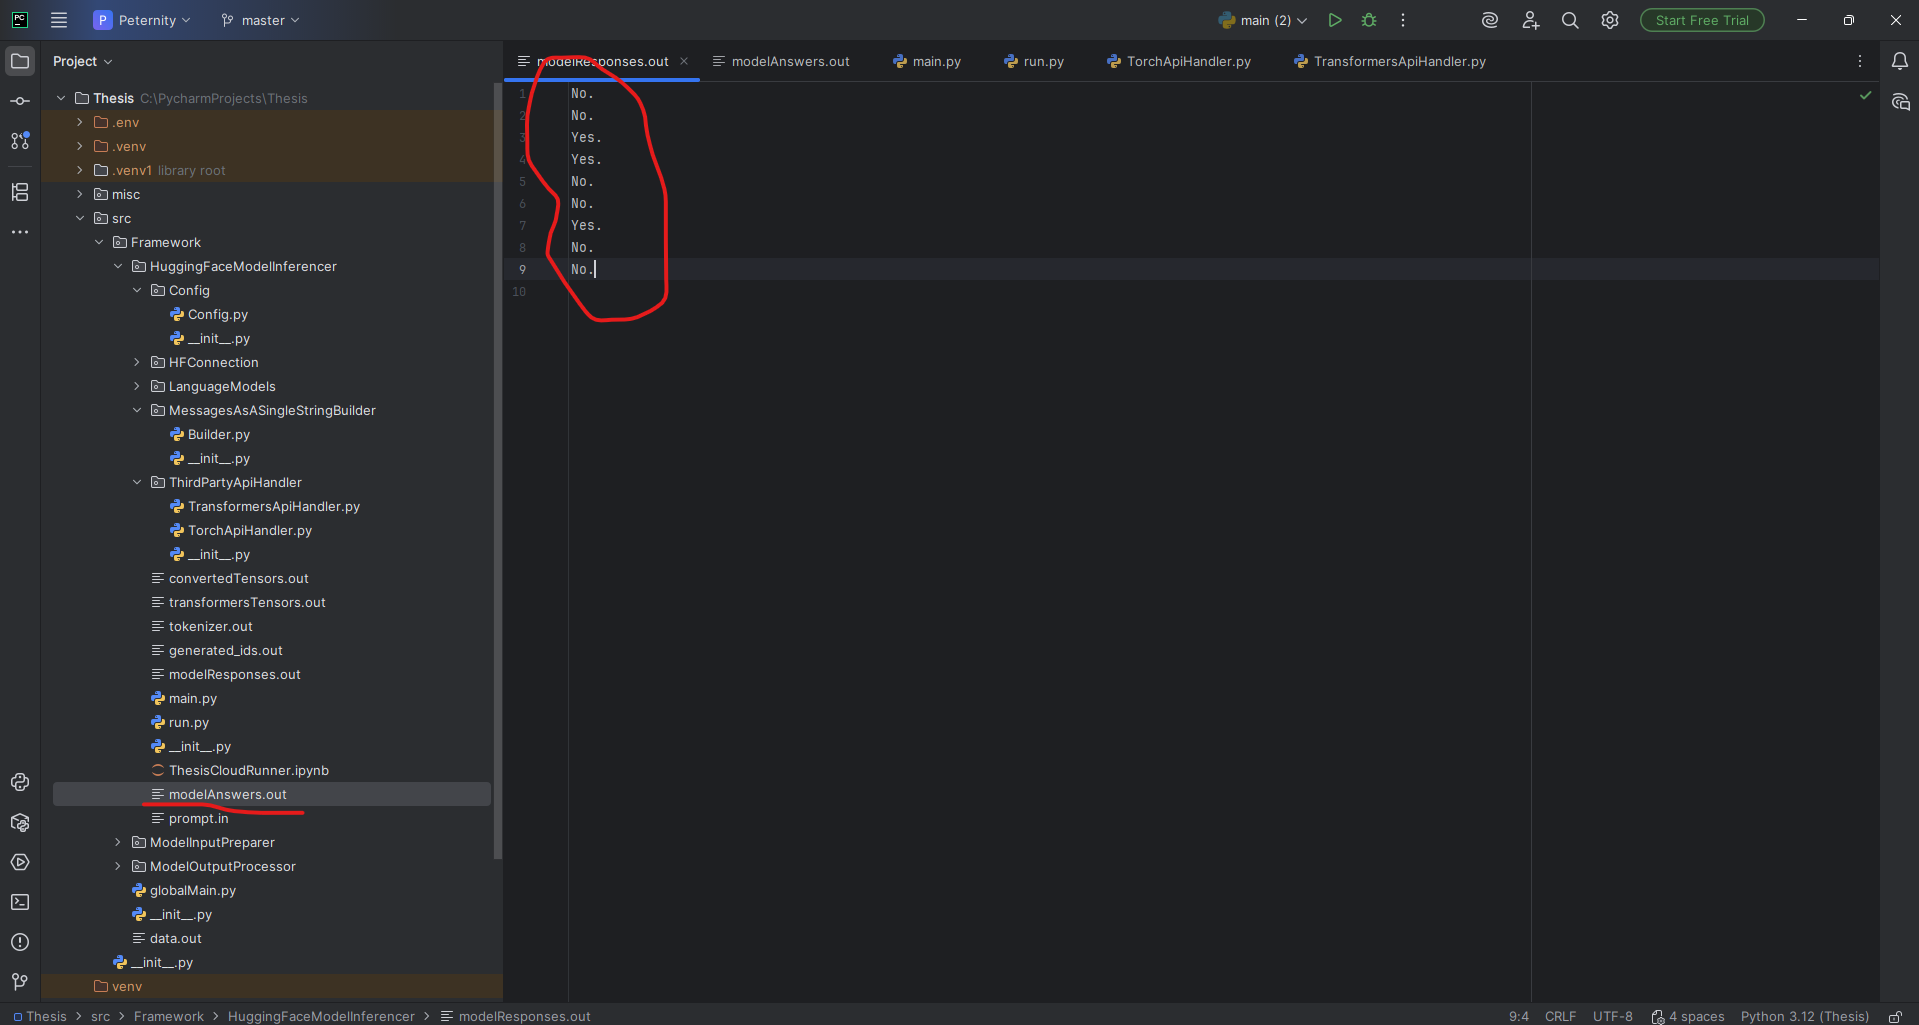
\includegraphics[keepaspectratio]{pelda}
                             \caption{Példa Válasz}
                             \label{fig:PeldaValasz}
                         \end{figure}


\chapter*{Nyilatkozat}
%Egy üres sort adunk a tartalomjegyzékhez:
\addtocontents{toc}{\ }
\addcontentsline{toc}{section}{Nyilatkozat}
%\hspace{\parindent}

% A nyilatkozat szövege más titkos és nem titkos dolgozatok esetében.
% Csak az egyik tipusú myilatokzatnak kell a dolgozatban szerepelni
% A ponok helyére az adatok értelemszerûen behelyettesídendõk es
% a szakdolgozat /diplomamunka szo megfeleloen kivalasztando.


%A nyilatkozat szövege TITKOSNAK NEM MINÕSÍTETT dolgozatban a következõ:
%A pontokkal jelölt szövegrészek értelemszerûen a szövegszerkesztõben és
%nem kézzel helyettesítendõk:

\noindent
Alulírott Fábián Bernát, programtervező informatikus BSc szakos hallgató, kijelentem, hogy a dolgozatomat a Szegedi Tudományegyetem Informatikai Intézet Számítógépes Algoritmusok és Mesterséges Intelligencia Tanszékén készítettem, a programtervező informatikus BSc diploma megszerzése érdekében.

Kijelentem, hogy a dolgozatot más szakon korábban nem védtem meg, saját munkám eredménye, és csak a hivatkozott forrásokat (szakirodalom, eszközök, stb.) használtam fel.

Tudomásul veszem, hogy szakdolgozatomat / diplomamunkámat a Szegedi Tudományegyetem Informatikai Intézet könyvtárában, a helyben olvasható könyvek között helyezik el.

\vspace*{2cm}

\begin{tabular}{lc}
	Szeged, \today\
	\hspace{2cm} & \makebox[6cm]{\dotfill} \\
	             & aláírás              \\
\end{tabular}

\vspace*{4cm}




\chapter*{Köszönetnyilvánítás}
\addcontentsline{toc}{section}{Köszönetnyilvánítás}

Ezúton szeretnék köszönetet mondani a családomnak, barátaimnak, tanítóimnak, tanáraimnak és egyetemi tanáraimnak, akik végigkísértek utamon és támogattak tanulmányaim alatt. Köszönetet szeretnék továbbá nyilvánítani szüleimnek, testvéreimnek és barátaimnak, hogy mindenben támogattak.

Végül, de nem utolsó sorban köszönetet szeretnék mondani \textbf{témavezetőmnek, Berend Gábornak}, hogy konzulensként és témavezetőként segített a szakdolgozatom megírásában.


%% Az itrodalomjegyzek keszitheto a BibTeX segedprogrammal:
%\bibliography{diploma}
%\bibliographystyle{plain}
\bibliographystyle{plainnat}
\bibliography{references}
% Journal Articles
@article{miller1994wordnet,
  title = {{WordNet}: A Lexical Database for {English}},
  author = {Miller, George A.},
  booktitle = {{H}uman {L}anguage {T}echnology: Proceedings of a Workshop held at {P}lainsboro, {N}ew {J}ersey, {M}arch 8-11, 1994},
  year = {1994},
  url = {https://aclanthology.org/H94-1111/}
}

@article{sokolova2009systematic,
  title = {A systematic analysis of performance measures for classification tasks},
  author = {Sokolova, Marina and Lapalme, Guy},
  journal = {Information Processing \& Management},
  volume = {45},
  number = {4},
  pages = {427--437},
  year = {2009},
  issn = {0306-4573},
  doi = {10.1016/j.ipm.2009.03.002},
  url = {https://www.sciencedirect.com/science/article/pii/S0306457309000259},
  keywords = {Performance evaluation, Machine Learning, Text classification}
}

@article{tan2024terms,
  title = {When the Terms of Service Change to Make Way for {A.I.} Training},
  author = {Tan, Eli},
  journal = {The New York Times},
  year = {2024},
  month = {6},
  day = {26},
  url = {https://www.nytimes.com/2024/06/26/technology/terms-service-ai-training.html}
}

@article{wolf2019huggingface,
  title = {{HuggingFace's} Transformers: State-of-the-art Natural Language Processing},
  author = {Wolf, Thomas and Debut, Lysandre and Sanh, Victor and Chaumond, Julien and Delangue, Clément and Moi, Anthony and Cistac, Pierric and Rault, Tim and Louf, Rémi and Funtowicz, Morgan and Davison, Joe and Shleifer, Sam and von Platen, Patrick and Ma, Clara and Jernite, Yacine and Plu, Julien and Xu, Canwen and Le Scao, Teven and Gugger, Sylvain and Drame, Mariama and Lhoest, Quentin and Rush, Alexander M.},
  journal = {arXiv preprint arXiv:1910.03771},
  year = {2019},
  url = {https://arxiv.org/abs/1910.03771}
}

% Conference Proceedings
@inproceedings{bird2004nltk,
  title = {{NLTK}: The Natural Language Toolkit},
  author = {Bird, Steven and Loper, Edward},
  booktitle = {Proceedings of the {ACL} Interactive Poster and Demonstration Sessions},
  month = jul,
  year = {2004},
  address = {Barcelona, Spain},
  publisher = {Association for Computational Linguistics},
  url = {https://aclanthology.org/P04-3031/},
  pages = {214--217}
}

@inproceedings{holtzman2020curious,
  title = {The Curious Case of Neural Text Degeneration},
  author = {Holtzman, Ari and Buys, Jan and Du, Li and Forbes, Maxwell and Choi, Yejin},
  booktitle = {Proceedings of the 8th International Conference on Learning Representations (ICLR)},
  year = {2020},
  url = {https://arxiv.org/abs/1904.09751},
  eprint = {1904.09751},
  archivePrefix = {arXiv}
}

@inproceedings{lesk1986automatic,
  title = {Automatic Sense Disambiguation Using Machine Readable Dictionaries: How to Tell a Pine Cone from an Ice Cream Cone},
  author = {Lesk, Michael E.},
  booktitle = {Proceedings of the 5th Annual International Conference on Systems Documentation (SIGDOC '86)},
  pages = {24--26},
  year = {1986},
  address = {New York, NY, USA},
  publisher = {ACM},
  url = {https://dl.acm.org/doi/10.1145/318723.318728}
}

@inproceedings{pilehvar2019wic,
  title = {{WiC}: the Word-in-Context Dataset for Evaluating Context-Sensitive Meaning Representations},
  author = {Pilehvar, Mohammad Taher and Camacho-Collados, Jose},
  booktitle = {Proceedings of the 2019 Conference of the North {A}merican Chapter of the Association for Computational Linguistics: Human Language Technologies, Volume 1 (Long and Short Papers)},
  month = jun,
  year = {2019},
  address = {Minneapolis, Minnesota},
  publisher = {Association for Computational Linguistics},
  url = {https://aclanthology.org/N19-1128/},
  doi = {10.18653/v1/N19-1128},
  pages = {1267--1273}
}

% ArXiv Preprints and Technical Reports
@misc{breit2021wictsv,
  title = {{WiC-TSV}: An Evaluation Benchmark for Target Sense Verification of Words in Context},
  author = {Breit, Anna and Revenko, Artem and Rezaee, Kiamehr and Pilehvar, Mohammad Taher and Camacho-Collados, Jose},
  year = {2021},
  eprint = {2004.15016},
  archivePrefix = {arXiv},
  primaryClass = {cs.CL},
  url = {https://arxiv.org/abs/2004.15016}
}

@misc{chiang2024chatbot,
  title = {Chatbot Arena: An Open Platform for Evaluating {LLMs} by Human Preference},
  author = {Chiang, Wei-Lin and Zheng, Lianmin and Sheng, Ying and Angelopoulos, Anastasios Nikolas and Li, Tianle and Li, Dacheng and Zhang, Hao and Zhu, Banghua and Jordan, Michael and Gonzalez, Joseph E. and Stoica, Ion},
  year = {2024},
  eprint = {2403.04132},
  archivePrefix = {arXiv},
  primaryClass = {cs.AI},
  url = {https://arxiv.org/abs/2403.04132}
}

@misc{raganato2020xlwic,
  title = {{XL-WiC}: A Multilingual Benchmark for Evaluating Semantic Contextualization},
  author = {Raganato, Alessandro and Pasini, Tommaso and Camacho-Collados, Jose and Pilehvar, Mohammad Taher},
  year = {2020},
  eprint = {2010.06478},
  archivePrefix = {arXiv},
  primaryClass = {cs.CL},
  url = {https://arxiv.org/abs/2010.06478}
}

@misc{sarlin2020superglue,
  title = {{SuperGlue}: Learning Feature Matching with Graph Neural Networks},
  author = {Sarlin, Paul-Edouard and DeTone, Daniel and Malisiewicz, Tomasz and Rabinovich, Andrew},
  year = {2020},
  eprint = {1911.11763},
  archivePrefix = {arXiv},
  primaryClass = {cs.CV},
  url = {https://arxiv.org/abs/1911.11763}
}

@misc{wang2020superglue,
  title = {{SuperGLUE}: A Stickier Benchmark for General-Purpose Language Understanding Systems},
  author = {Wang, Alex and Pruksachatkun, Yada and Nangia, Nikita and Singh, Amanpreet and Michael, Julian and Hill, Felix and Levy, Omer and Bowman, Samuel R.},
  year = {2020},
  eprint = {1905.00537},
  archivePrefix = {arXiv},
  primaryClass = {cs.CL},
  url = {https://arxiv.org/abs/1905.00537}
}

% Software and Models
@misc{anthropic2025api,
  title = {Client {SDKs} - {Anthropic} {API}},
  author = {Anthropic},
  year = {2025},
  howpublished = {\url{https://docs.anthropic.com/en/api/client-sdks}}
}

@misc{berend2025phi,
  title = {11\_phi.ipynb},
  author = {Berend, Gábor},
  year = {2025},
  note = {Google Colab jegyzetfüzet},
  howpublished = {\url{https://colab.research.google.com/drive/1GQRiTDNWwNPP_PPARYd1swY1Oiai9Ey_}},
  urldate = {2025-05-23}
}

@misc{gemma22b2024,
  title = {Gemma-2-2b-it},
  author = {Google},
  howpublished = {\url{https://huggingface.co/google/gemma-2-2b-it}},
  year = {2024}
}

@misc{openai2025api,
  title = {{OpenAI} {API} Documentation Overview},
  author = {OpenAI},
  year = {2025},
  url = {https://platform.openai.com/docs/overview}
}

@misc{peters2004zen,
  title = {{PEP} 20 -- The Zen of Python},
  author = {Peters, Tim},
  year = {2004},
  howpublished = {\url{https://peps.python.org/pep-0020/}},
  note = {Python Enhancement Proposal}
}

@misc{phi4mini2024,
  title = {Phi-4-mini-instruct},
  author = {Microsoft},
  howpublished = {\url{https://huggingface.co/microsoft/Phi-4-mini-instruct}},
  year = {2024}
}

@misc{qwen15chat2024,
  title = {Qwen1.5-1.8B-Chat},
  author = {Qwen},
  howpublished = {\url{https://huggingface.co/Qwen/Qwen1.5-1.8B-Chat}},
  year = {2024}
}

% Online Resources and Web Articles
@online{oloruntoba2024solid,
  title = {{SOLID}: The First 5 Principles of Object Oriented Design},
  author = {Oloruntoba, Samuel and Walia, Anish Singh},
  year = {2024},
  month = apr,
  url = {https://www.digitalocean.com/community/conceptual-articles/s-o-l-i-d-the-first-five-principles-of-object-oriented-design}
}

@online{springboard2023gpt3,
  title = {{OpenAI} {GPT-3}: Everything You Need to Know},
  author = {Springboard},
  year = {2023},
  url = {https://www.springboard.com/blog/data-science/machine-learning-gpt-3-open-ai/}
}

@online{verge2023nytai,
  title = {The New York Times prohibits using its content to train {AI} models},
  author = {The Verge},
  year = {2023},
  url = {https://www.theverge.com/2023/8/14/23831109/the-new-york-times-ai-web-scraping-rules-terms-of-service}
}

@online{manrai2020covid,
  author       = {Arjun K. Manrai and Kenneth D. Mandl},
  title        = {Covid-19 testing: overcoming challenges in the next phase of the epidemic},
  year         = {2020},
  month        = mar,
  day          = {31},
  url          = {https://www.statnews.com/2020/03/31/covid-19-overcoming-testing-challenges/},
  note         = {Accessed: 2025-05-25}
}

@book{martin2008cleancode,
  title        = {Clean Code: A Handbook of Agile Software Craftsmanship},
  author       = {Martin, Robert C.},
  year         = {2008},
  publisher    = {Prentice Hall},
  address      = {Upper Saddle River, NJ, USA},
  isbn         = {978-0-13-235088-4}
}

[1] Mohammad Taher Pilehvar és Jose Camacho-Collados. „WiC: the Word-in-Context
Dataset for Evaluating Context-Sensitive Meaning Representations”. Proceedings
of the 2019 Conference of the North American Chapter of the Association for
Computational Linguistics: Human Language Technologies, Volume 1 (Long and
Short Papers). Szerk. Jill Burstein, Christy Doran és Thamar Solorio. Minneapolis,
Minnesota: Association for Computational Linguistics, 2019. jún., 1267–1273. old.
DOI: 10.18653/v1/N19-1128. URL: https://aclanthology.org/
N19-1128/.
[2] Michael E. Lesk. „Automatic Sense Disambiguation Using Machine Readable Dictionaries: How to Tell a Pine Cone from an Ice Cream Cone”. Proceedings of the
5th Annual International Conference on Systems Documentation (SIGDOC ’86).
New York, NY, USA: ACM, 1986, 24–26. old. URL: https://dl.acm.org/
doi/10.1145/318723.318728.
[3] Paul-Edouard Sarlin és tsai. SuperGlue: Learning Feature Matching with Graph Neural Networks. 2020. arXiv: 1911.11763 [cs.CV]. URL: https://
arxiv.org/abs/1911.11763.
[4] Alex Wang és tsai. SuperGLUE: A Stickier Benchmark for General-Purpose Language Understanding Systems. 2020. arXiv: 1905.00537 [cs.CL]. URL: https:
//arxiv.org/abs/1905.00537.
[5] Wei-Lin Chiang és tsai. Chatbot Arena: An Open Platform for Evaluating LLMs
by Human Preference. 2024. arXiv: 2403 . 04132 [cs.AI]. URL: https :
//arxiv.org/abs/2403.04132.
[6] Springboard. OpenAI GPT-3: Everything You Need to Know. 2023. URL: https:
//www.springboard.com/blog/data-science/machine-learninggpt-3-open-ai/.
[7] The Verge. The New York Times prohibits using its content to train AI models. 2023.
URL: https://www.theverge.com/2023/8/14/23831109/thenew-york-times-ai-web-scraping-rules-terms-of-service.
[8] Eli Tan. „When the Terms of Service Change to Make Way for A.I. Training”. The
New York Times (2024. jún.). URL: https://www.nytimes.com/2024/
06/26/technology/terms-service-ai-training.html.
[9] Thomas Wolf és tsai. „HuggingFace’s Transformers: State-of-the-art Natural Language Processing”. arXiv preprint arXiv:1910.03771 (2019). URL: https : / /
arxiv.org/abs/1910.03771.
[10] Ari Holtzman és tsai. „The Curious Case of Neural Text Degeneration”. Proceedings of the 8th International Conference on Learning Representations (ICLR).
2020. arXiv: 1904 . 09751. URL: https : / / arxiv . org / abs / 1904 .
09751.
[11] Gábor Berend. 11\_phi.ipynb. https://colab.research.google.com/
drive/1GQRiTDNWwNPP\_PPARYd1swY1Oiai9Ey\_. Google Colab jegyzetfüzet. 2025. (Elérés dátuma 2025. 05. 23.).
[12] Microsoft. Phi-4-mini-instruct. https://huggingface.co/microsoft/
Phi-4-mini-instruct. 2023.
[13] Google. Gemma-2-2b-it. https://huggingface.co/google/gemma2-2b-it. 2023.
[14] Qwen. Qwen1.5-1.8B-Chat. https://huggingface.co/Qwen/Qwen1.
5-1.8B-Chat. 2023.
[15] Steven Bird és Edward Loper. „NLTK: The Natural Language Toolkit”. Proceedings of the ACL Interactive Poster and Demonstration Sessions. Barcelona, Spain:
Association for Computational Linguistics, 2004. júl., 214–217. old. URL: https:
//aclanthology.org/P04-3031/.
[16] George A. Miller. „WordNet: A Lexical Database for English”. Human Language
Technology: Proceedings of a Workshop held at Plainsboro, New Jersey, March
8-11, 1994. 1994. URL: https://aclanthology.org/H94-1111/.
[17] Tim Peters. PEP 20 – The Zen of Python. https://peps.python.org/
pep-0020/. Python Enhancement Proposal. 2004.
[18] Samuel Oloruntoba és Anish Singh Walia. SOLID: The First 5 Principles of Object
Oriented Design. 2024. ápr. URL: https : / / www . digitalocean . com /
community / conceptual - articles / s - o - l - i - d - the - first -
five-principles-of-object-oriented-design.
[19] OpenAI. OpenAI API Documentation Overview. 2025. URL: https://platform.
openai.com/docs/overview.
[20] Anthropic. Client SDKs - Anthropic API. https://docs.anthropic.com/
en/api/client-sdks. 2025.
[21] Alessandro Raganato és tsai. XL-WiC: A Multilingual Benchmark for Evaluating Semantic Contextualization. 2020. arXiv: 2010 . 06478 [cs.CL]. URL:
https://arxiv.org/abs/2010.06478.
[22] Anna Breit és tsai. WiC-TSV: An Evaluation Benchmark for Target Sense Verification of Words in Context. 2021. arXiv: 2004.15016 [cs.CL]. URL: https:
//arxiv.org/abs/2004.15016.


%VAGY "kézzel" a következõ módon:

\begin{thebibliography}{9}
%10-nél kevesebb hivatkozás esetén

%\begin{thebibliography}{99}
% 10-nél több hivatkozás esetén

\addcontentsline{toc}{section}{Irodalomjegyzék}

%Elso szerzok vezetekneve alapjan ábécérendben rendezve.


%folyóirat cikk: szerzok(k), a folyóirat neve kiemelve,
%az evfolyam felkoveren, zarojelben az evszam, vegul az oldalszamok es pont.
\bibitem{Gischer}
J. L. Gischer,
The equational theory of pomsets.
\emph{Theoret. Comput. Sci.}, \textbf{61}(1988), 199--224.

%könyv (szerzo(k), a könyv neve kiemelve, utana a kiado, a kiado szekhelye, az evszam es pont.)
\bibitem{Pin}
J.-E. Pin,
\emph{Varieties of Formal Languages},
Plenum Publishing Corp., New York, 1986.





\end{thebibliography}

\chapter*{Elektronikus mellékletek}
\addcontentsline{toc}{section}{Nyilatkozat}

\begin{itemize}
\item A keretrendszeren GitHubról a\\ \href{https://github.com/Fabbernat/Thesis}{GitHub/Fabbernat/Thesis}\\ repozitóriumban található.

\item A szakdolgozat pdf forráskódja a \href{https://github.com/Fabbernat/Thesis-paper}{GitHub/Fabbernat/Thesis-paper}\\ repozitóriumban található.

    \item
\label{att:colab}
A modelleket futtató Google Colab jegyzetfüzetem (elavult):
\href{https://colab.research.google.com/drive/1yA8IAd5z2oreKUXha-16Du2YrNhemNiU?usp=sharing}{ezen a linken}  található.

\item A nyelvi modellek tesztelésének és kiértékelésének régi eredményei a
\href{https://docs.google.com/spreadsheets/d/1y49lg52LHVFmTom-0ibCqYqWA1pKKhiUny-Pf3KVTIg/edit?usp=sharing}{Generative Language Models}
táblázatban tekinthető meg.
\end{itemize}


\end{document}
